\documentclass[a4paper]{article}
\usepackage{a4wide,amssymb,epsfig,latexsym,multicol,array,hhline,fancyhdr}
\usepackage{vntex}
\usepackage{amsmath}
\usepackage{lastpage}
\usepackage[lined,boxed,commentsnumbered]{algorithm2e}
\usepackage{enumerate}
\usepackage{color}
\usepackage{graphicx}							% Standard graphics package
\usepackage{array}
\usepackage{tabularx, caption}
\usepackage{multirow}
\usepackage{multicol}
\usepackage{rotating}
\usepackage{multicol}
\usepackage{graphics}
\usepackage{geometry}
\usepackage{setspace}
\usepackage{epsfig}
\usepackage{tikz}
\usepackage{tkz-graph}
\usetikzlibrary{arrows.meta}
\usepackage{enumitem}
\usepackage{algorithmic}
\usepackage{xcolor}
\usepackage{algorithm}
\usetikzlibrary{arrows,snakes,backgrounds}
\usepackage{hyperref}
\hypersetup{urlcolor=blue,linkcolor=black,citecolor=black,colorlinks=true} 
%\usepackage{pstcol} 								% PSTricks with the standard color package
\usepackage{listings}

\newtheorem{theorem}{{\bf Theorem}}
\newtheorem{property}{{\bf Property}}
\newtheorem{proposition}{{\bf Proposition}}
\newtheorem{corollary}[proposition]{{\bf Corollary}}
\newtheorem{lemma}[proposition]{{\bf Lemma}}

\AtBeginDocument{\renewcommand*\contentsname{Contents}}
\AtBeginDocument{\renewcommand*\refname{References}}
%\usepackage{fancyhdr}
\setlength{\headheight}{40pt}
\pagestyle{fancy}
\fancyhead{} % clear all header fields
\fancyhead[L]{
 \begin{tabular}{rl}
    \begin{picture}(25,15)(0,0)
    \put(0,-8){
\includegraphics[width=8mm, height=8mm]{assets/hcmut.png}}
    %\put(0,-8){\epsfig{width=10mm,figure=hcmut.eps}}
   \end{picture}&
	%
\includegraphics[width=8mm, height=8mm]{assets/hcmut.png} & %
	\begin{tabular}{l}
		\textbf{\bf \ttfamily University of Technology, Ho Chi Minh City}\\
		\textbf{\bf \ttfamily Faculty of Computer Science and Engineering}
	\end{tabular} 	
 \end{tabular}
}
\fancyhead[R]{
	\begin{tabular}{l}
		\tiny \bf \\
		\tiny \bf 
	\end{tabular}  }
\fancyfoot{} % clear all footer fields
\fancyfoot[L]{\scriptsize \ttfamily Assignment for Advanced system architectures}
\fancyfoot[R]{\scriptsize \ttfamily Page {\thepage}/\pageref{LastPage}}
\renewcommand{\headrulewidth}{0.3pt}
\renewcommand{\footrulewidth}{0.3pt}


%%%
\setcounter{secnumdepth}{4}
\setcounter{tocdepth}{3}
\makeatletter
\newcounter {subsubsubsection}[subsubsection]
\renewcommand\thesubsubsubsection{\thesubsubsection .\@alph\c@subsubsubsection}
\newcommand\subsubsubsection{\@startsection{subsubsubsection}{4}{\z@}%
                                     {-3.25ex\@plus -1ex \@minus -.2ex}%
                                     {1.5ex \@plus .2ex}%
                                     {\normalfont\normalsize\bfseries}}
\newcommand*\l@subsubsubsection{\@dottedtocline{3}{10.0em}{4.1em}}
\newcommand*{\subsubsubsectionmark}[1]{}
\makeatother

% Define a custom color
\definecolor{codegreen}{rgb}{0,0.6,0}
\definecolor{codegray}{rgb}{0.5,0.5,0.5}
\definecolor{codepurple}{rgb}{0.58,0,0.82}
\definecolor{backcolour}{rgb}{0.95,0.95,0.92}

% Define a custom style
\lstdefinestyle{myStyle}{
    backgroundcolor=\color{backcolour},   
    commentstyle=\color{codegreen},
    keywordstyle=\color{magenta},
    numberstyle=\tiny\color{codegray},
    stringstyle=\color{codepurple},
    basicstyle=\ttfamily\footnotesize,
    breakatwhitespace=false,         
    breaklines=true,                 
    keepspaces=true,                 
    numbers=left,       
    numbersep=5pt,                  
    showspaces=false,                
    showstringspaces=false,
    showtabs=false,                  
    tabsize=2,
}
% Use \lstset to make myStyle the global default
\lstset{style=myStyle}

\begin{document}

\begin{titlepage}
\begin{center}
VIETNAM NATIONAL UNIVERSITY, HO CHI MINH CITY \\
UNIVERSITY OF TECHNOLOGY \\
FACULTY OF COMPUTER SCIENCE AND ENGINEERING
\end{center}

\vspace{1cm}

\begin{figure}[h!]
\begin{center}

\includegraphics[width=3cm]{assets/hcmut.png}
\end{center}
\end{figure}

\vspace{1cm}


\begin{center}
\begin{tabular}{c}
\multicolumn{1}{c}{\textbf{{\Large ADVANCED SYSTEM ARCHITECTURES(CO5260)}}}\\

~~\\
\hline
\\
\multicolumn{1}{l}{\textbf{{\Large Assignment}}}\\
\\
\textbf{{\Huge AI Chips }}
\\
\textbf{{\Huge }}\\
\\
\hline
\end{tabular}
\end{center}

\vspace{1.5cm}

\begin{table}[h]
\begin{tabular}{rrl}
\hspace{5 cm} & Advisor: & Assoc.Prof. Dr. Trần Ngọc Thịnh \\ 
&& Assoc.Prof. Dr. Phạm Hoàng Anh \\
& Students: &1. Trần Hoài Tâm - 2470743 \\
&&2. Võ Minh Chánh - 2470501 \\
&&3. Nguyễn Thành Nhân - 2491089 \\
&&4. Nguyễn Thanh Minh Đức - 2470734 \\
&&5. Bùi Tiến Đức - 2498016 \\
&&6. Trương Vĩnh Phước - 2470506 \\
&&7. Phạm Minh Tú - 2470511 \\
&&8. Nguyễn Đông Dũng - 2470568 \\
&&9. Cao Nguyễn Minh Hiếu - 2470575 \\
&&10. Lê Quang Trung - 2470746 \\
&&11. Nguyễn Hữu Trưởng - 2470573 \\
&&12. Võ Thị Bích Phượng - 2470570 \\


\end{tabular}
\end{table}

\begin{center}
{\footnotesize HO CHI MINH CITY, MARCH 2025}
\end{center}
\end{titlepage}


%\thispagestyle{empty}

\newpage
\tableofcontents
\newpage

%%%%%%%%%%%%%%%%%%%%%%%%%%%%%%%%%
\section{Introduction}
Với sự phát triển của ngành công nghiệp video ngắn và sự xuất hiện của kỷ nguyên dữ liệu lớn cùng Internet vạn vật (IoTs), lượng dữ liệu mà con người tạo ra trong những năm gần đây đã tăng trưởng bùng nổ, cung cấp một nền tảng dữ liệu vững chắc cho sự phát triển của trí tuệ nhân tạo (AI). Là công nghệ cốt lõi và hướng nghiên cứu để hiện thực hóa trí tuệ nhân tạo, học sâu dựa trên mạng nơ-ron đã đạt được những kết quả tốt trong nhiều lĩnh vực như nhận diện giọng nói [1–3], xử lý hình ảnh [4–6] và xử lý ngôn ngữ tự nhiên [7–9]. Các nền tảng phổ biến để tăng tốc học sâu bao gồm bộ xử lý trung tâm (CPU), bộ xử lý đồ họa (GPU), mảng cổng lập trình được tại hiện trường (FPGA) và mạch tích hợp dành riêng cho ứng dụng (ASIC).

Trong số đó, CPU sử dụng kiến trúc Von Neumann và việc thực thi chương trình trong lĩnh vực học sâu của trí tuệ nhân tạo là ít, trong khi nhu cầu tính toán dữ liệu lại tương đối lớn. Do đó, việc triển khai các thuật toán AI bằng CPU có một hạn chế cấu trúc tự nhiên—tức là CPU mất rất nhiều thời gian để đọc và phân tích dữ liệu hoặc lệnh. Nói chung, không thể cải thiện tốc độ thực thi lệnh một cách không giới hạn bằng cách tăng tần số CPU và băng thông bộ nhớ mà không có giới hạn.

Ở cấp độ cao, điều này có nghĩa là các nhà thiết kế hệ thống phải đối mặt với hai lựa chọn. Một là chọn một hệ thống dị hợp và tích hợp một số lượng lớn chip tăng tốc ASIC vào hệ thống để xử lý các loại vấn đề khác nhau. Hai là chọn một chip duy nhất để xử lý càng nhiều loại thuật toán càng tốt. Giải pháp FPGA thuộc loại thứ hai vì FPGA cung cấp logic có thể tái cấu hình không giới hạn, trong khi FPGA có thể cập nhật chức năng logic chỉ trong vài trăm mili giây, và chúng ta có thể thiết kế các bộ tăng tốc cho từng thuật toán. Sự thỏa hiệp duy nhất là các bộ tăng tốc này sử dụng logic lập trình thay vì cổng cố định, nhưng điều này cũng có nghĩa là chúng ta có thể tận dụng tính linh hoạt của FPGA để giúp tiết kiệm chi phí phát triển hơn nữa.

Hiện nay, các yêu cầu tính toán trí tuệ nhân tạo được đại diện bởi học sâu chủ yếu sử dụng GPU, FPGA và các chip chung hiện có khác phù hợp với tính toán song song để đạt được sự tăng tốc. Nhờ đặc điểm song song cao, tần số cao và băng thông cao, GPU có thể song song hóa các phép toán và rút ngắn đáng kể thời gian vận hành của mô hình. Nhờ khả năng tính toán mạnh mẽ, nó hiện chủ yếu được sử dụng để xử lý các tác vụ tính toán quy mô lớn. Các thuật toán học sâu tăng tốc bằng GPU đã được ứng dụng rộng rãi và đạt được những kết quả đáng kể.
\subsection{Sự phát triển của mạng no-ron}

Giai đoạn từ năm 1943 đến 1958 được coi là giai đoạn đề xuất mô hình, và làn sóng perceptron được đề xuất vào năm 1958 kéo dài khoảng 10 năm. Khi ngày càng nhiều học giả tham gia vào hướng nghiên cứu này, một số học giả dần phát hiện ra những hạn chế của mô hình perceptron. Với việc xuất bản cuốn \textit{Perceptron} của M. Minsky vào năm 1969, mạng nơ-ron bị đẩy xuống đáy, dẫn đến "thời kỳ đình trệ" của mạng nơ-ron từ năm 1969 đến 1980.
% \begin{figure}[H]
%      \centering
%      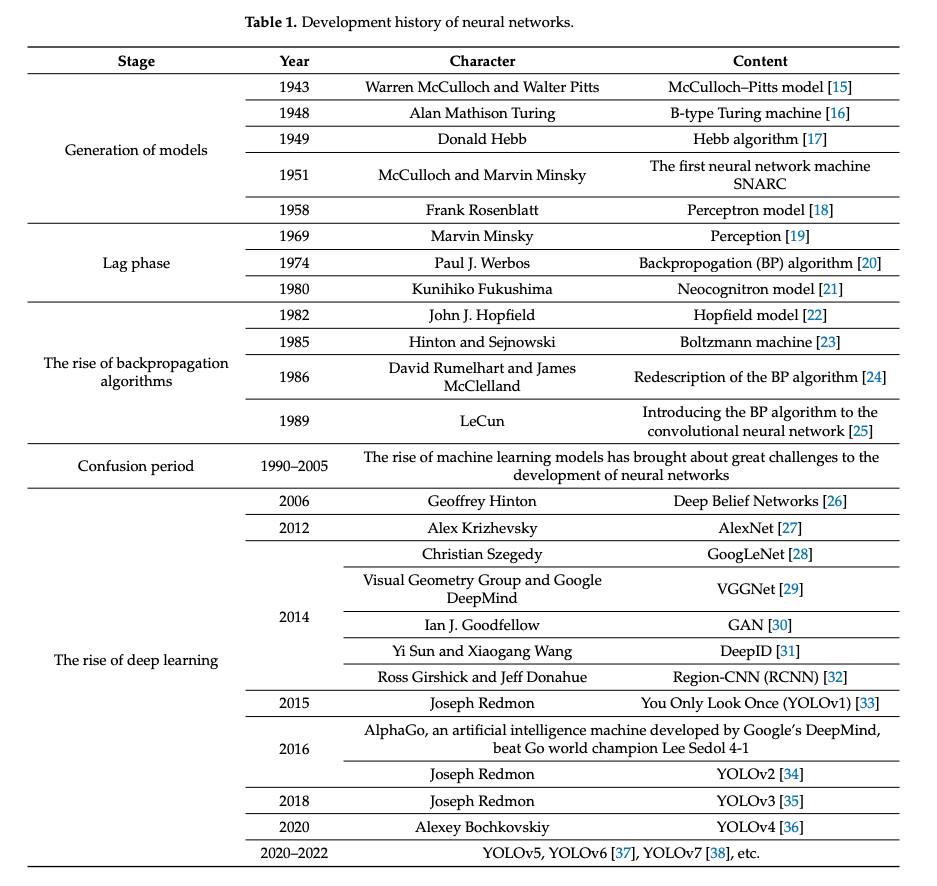
\includegraphics[scale =0.45]{assets/table-1.png}
%      \caption{Lịch sử phát triển của nơ-ron network}
%      \label{fig:2ss}
%  \end{figure}
 
Sau năm 1980, ngày càng nhiều học giả chú ý đến thuật toán lan truyền ngược, điều này đã mở lại tư duy cho các nhà nghiên cứu và khởi đầu một mùa xuân khác cho sự phát triển của mạng nơ-ron.

Sau đó, trong một thời gian dài, các học giả không đạt được kết quả đột phá, chỉ làm việc dựa trên các nghiên cứu hiện có. Vào giữa những năm 1990, lý thuyết học thống kê và mô hình học máy được đại diện bởi máy vector hỗ trợ bắt đầu nổi lên. Ngược lại, cơ sở lý thuyết của mạng nơ-ron không rõ ràng, và các khó khăn về tối ưu hóa, khả năng giải thích kém cùng các nhược điểm khác trở nên nổi bật hơn; do đó, nghiên cứu mạng nơ-ron lại rơi vào giai đoạn thoái trào.

Cho đến năm 2006, Giáo sư Geoffrey Hinton, một chuyên gia về mạng nơ-ron tại Đại học Toronto, cùng các học trò của mình chính thức đề xuất khái niệm học sâu. Họ đã đề xuất mô hình mạng niềm tin sâu trong bài báo được công bố. Hinton và các cộng sự [26] phát hiện rằng mạng nơ-ron tiến tới đa tầng có thể được huấn luyện trước từng tầng. Nói cách khác, phương pháp huấn luyện trước không giám sát được sử dụng để cải thiện giá trị ban đầu của trọng số mạng, sau đó các trọng số được tinh chỉnh. Mô hình này đã khởi đầu làn sóng nghiên cứu về mạng nơ-ron sâu và mở đầu cho việc nghiên cứu và ứng dụng học sâu.

Hiện nay, các mô hình học sâu phổ biến bao gồm mạng nơ-ron sâu (DNN), mạng nơ-ron tích chập (CNN), mạng nơ-ron hồi quy (RNN) và mạng đối kháng sinh tạo (GAN), cùng nhiều mô hình khác.
\subsection{How AI Chips Work}

%%%%%%%%%%%%%%%%%%%%%%%%%%%%%%%%%
\section{Cơ sở lý thuyết}
\subsection{Vector Processing}
\subsubsection{SIMD - Single Instruction, Multiple Data}
SIMD là một mô hình tính toán song song thuộc phân loại Flynn (Flynn's Taxonomy), được sử dụng để thực hiện cùng một lệnh (instruction) trên nhiều phần tử dữ liệu (data) cùng lúc. Cụ thể:
\begin{itemize}
\item \textbf{Single Instruction}: Một lệnh duy nhất được phát ra.
\item \textbf{Multiple Data}: Lệnh này được áp dụng đồng thời trên nhiều phần tử dữ liệu khác nhau.
\end{itemize}
% \begin{itemize}
 
% \end{itemize}

SIMD là một dạng của \textbf{data-level parallelism} (tính song song ở cấp độ dữ liệu), nghĩa là nó khai thác tính song song bằng cách xử lý nhiều phần tử dữ liệu cùng lúc, thay vì thực hiện nhiều lệnh khác nhau (như trong mô hình MIMD - Multiple Instruction, Multiple Data).
\begin{figure}[H]
     \centering
     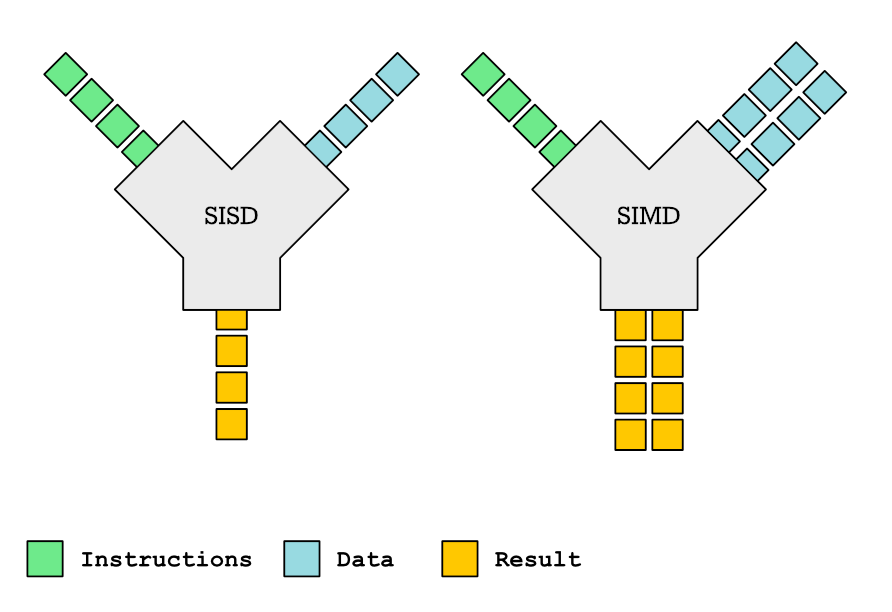
\includegraphics[scale=0.3]{assets/simd.png}
     \caption{SISD và SIMD}
     \label{fig:2ss}
 \end{figure}
 
\subsubsection{Vector Programming Model}
\paragraph{Tổng quan về Vector Programming Model} \leavevmode\\

Mô hình lập trình vector là cách mà các lập trình viên hoặc trình biên dịch tương tác với phần cứng của một máy vector. Nó cung cấp một tập hợp các tài nguyên (như thanh ghi vector) và lệnh (như lệnh vector arithmetic) để thực hiện các phép tính song song trên nhiều phần tử dữ liệu cùng lúc (theo kiểu SIMD - Single Instruction, Multiple Data). Mô hình này được thiết kế để:

\begin{itemize}
\item Tận dụng tính song song ở cấp độ dữ liệu (data-level parallelism).
\item Giảm chi phí điều khiển (control overhead) so với các mô hình scalar truyền thống.
\item Hỗ trợ các ứng dụng yêu cầu xử lý dữ liệu lớn, như tính toán khoa học, xử lý đồ họa, hoặc học máy.
\end{itemize}

\begin{figure}[H]
     \centering
     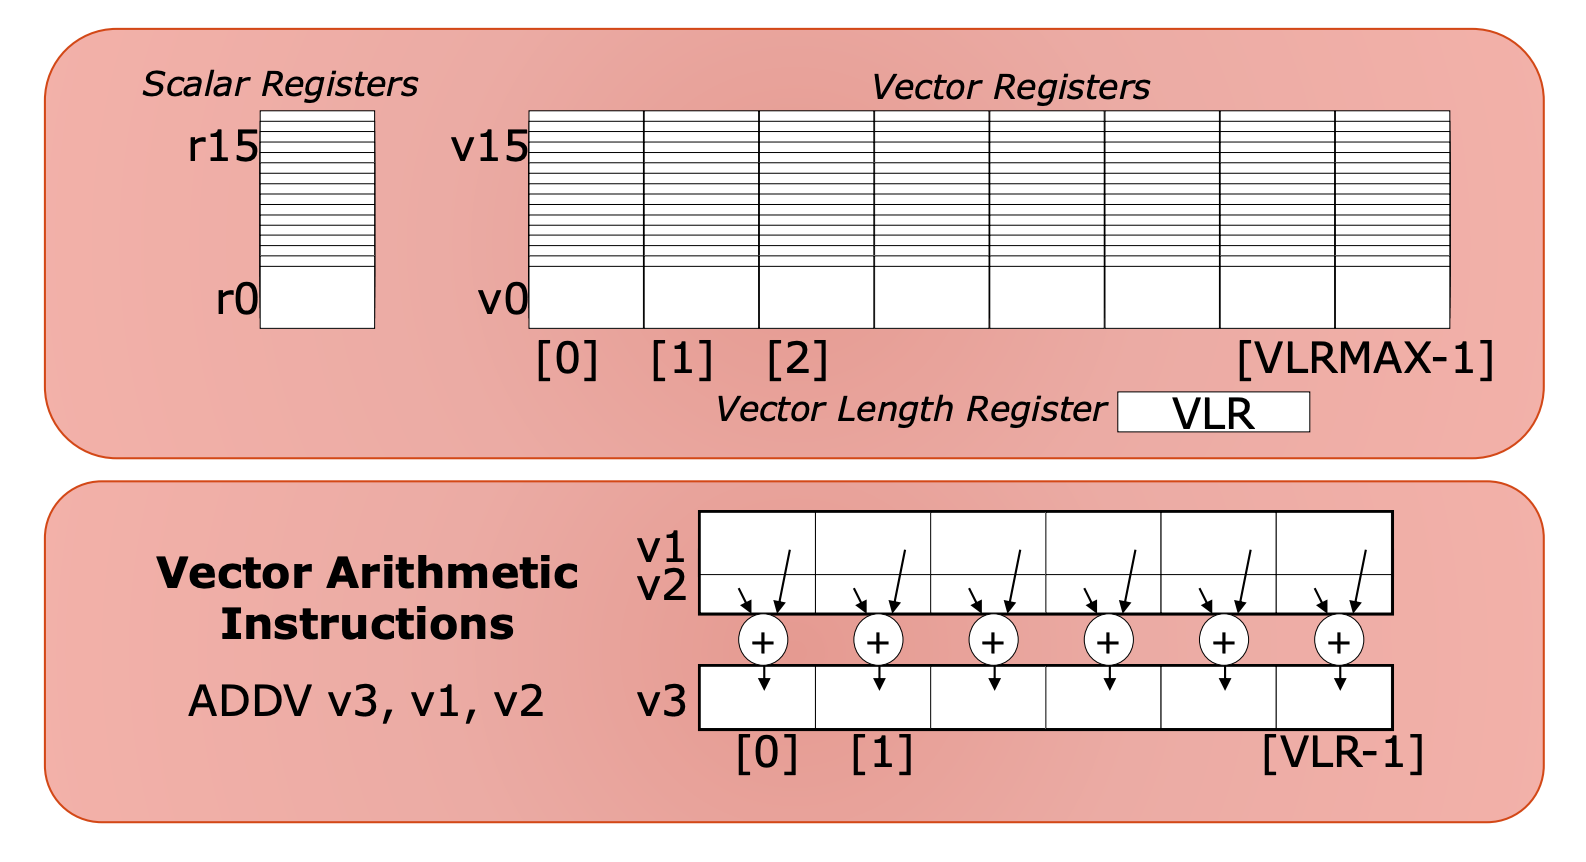
\includegraphics[scale =0.4]{assets/vector-programming-model.png}
     \caption{Vector programming model}
     \label{fig:2ss}
 \end{figure}

 Hình ảnh thể hiện một phần của kiến trúc lập trình vector, một mô hình được thiết kế để xử lý dữ liệu dạng mảng (vector) một cách hiệu quả. Cụ thể, nó bao gồm các thanh ghi scalar (r0 đến r15) dùng để lưu trữ các giá trị đơn lẻ như địa chỉ hay hằng số, và các thanh ghi vector (v0 đến v15) dùng để chứa các tập hợp dữ liệu lớn hơn, tức là các vector. Ngoài ra, còn có VLR, một thanh ghi đặc biệt quyết định số phần tử của vector sẽ được xử lý trong mỗi lệnh, và một ví dụ về lệnh vector là ADDV, thực hiện phép cộng giữa các vector. Tất cả các thành phần này phối hợp để tạo nên một hệ thống xử lý dữ liệu song song mạnh mẽ.

\paragraph{Thanh ghi Scalar (Scalar Registers)}\leavevmode\\

Thanh ghi scalar, được ký hiệu từ r0 đến r15 trong hình (tổng cộng 16 thanh ghi), là những thanh ghi thông thường mà ta thường thấy trong các kiến trúc máy tính cơ bản. Mỗi thanh ghi này chỉ lưu trữ được một giá trị đơn, gọi là giá trị scalar, chẳng hạn như một số nguyên hoặc một địa chỉ bộ nhớ. Chúng đóng vai trò như những "trợ thủ" trong việc điều khiển và hỗ trợ các phép tính vector. Ví dụ, r0 có thể chứa địa chỉ bắt đầu của một vector trong bộ nhớ, còn r1 có thể lưu giá trị stride, tức là khoảng cách giữa các phần tử liên tiếp trong vector đó. Nhờ tính đơn giản và linh hoạt, các thanh ghi scalar thường được dùng để quản lý vòng lặp, lưu trữ hằng số hoặc cung cấp thông tin đầu vào cho các lệnh vector, giúp quá trình xử lý dữ liệu trơn tru hơn.

\paragraph{Thanh ghi Vector (Vector Registers)}\leavevmode\\

Khác với thanh ghi scalar, các thanh ghi vector (v0 đến v15, cũng có 16 thanh ghi trong hình) được thiết kế đặc biệt để lưu trữ toàn bộ một vector, tức là một dãy các phần tử dữ liệu. Mỗi thanh ghi vector có thể chứa nhiều giá trị, từ phần tử đầu tiên [0] cho đến phần tử cuối cùng [VLRMAX-1], trong đó VLRMAX là độ dài tối đa mà phần cứng cho phép, ví dụ như 64 phần tử. Điều này có nghĩa là nếu VLRMAX là 64, thì một thanh ghi như v1 có thể chứa một dãy dữ liệu như [a0, a1, ..., a63], và v2 chứa [b0, b1, ..., b63]. Công dụng chính của chúng là lưu trữ dữ liệu để thực hiện các phép tính song song, cho phép máy tính xử lý nhiều phần tử cùng lúc thay vì từng phần tử một như cách truyền thống. Đây chính là điểm mạnh của lập trình vector, giúp tăng tốc độ xử lý đáng kể.

\paragraph{Thanh ghi Độ dài Vector (Vector Length Register - VLR)}\leavevmode\\

VLR là một thanh ghi đặc biệt, đóng vai trò như "người điều phối" trong mô hình lập trình vector. Nó lưu trữ độ dài hiện tại của vector mà các lệnh vector sẽ xử lý, với giá trị nằm trong khoảng từ 1 đến VLRMAX. Ví dụ, nếu VLR được đặt là 32, thì máy chỉ xử lý 32 phần tử đầu tiên của thanh ghi vector (từ [0] đến [31]), bỏ qua các phần tử còn lại dù thanh ghi có thể chứa tối đa 64 phần tử. Điều này mang lại sự linh hoạt lớn: không phải vector nào cũng cần xử lý hết độ dài tối đa, và VLR giúp máy thích nghi với các kích thước vector khác nhau mà không cần phải thêm dữ liệu giả (padding) để lấp đầy. Trong lập trình, khi một vòng lặp lớn được chia thành các đoạn nhỏ để vector hóa, VLR đặc biệt hữu ích ở đoạn cuối – nơi số phần tử còn lại thường nhỏ hơn VLRMAX. Chẳng hạn, nếu chỉ còn 10 phần tử cần xử lý, VLR được đặt thành 10 để đảm bảo xử lý đúng và đủ.

\paragraph{Lệnh Số học Vector (Vector Arithmetic Instructions)}\leavevmode\\

\begin{figure}[H]
    \centering
    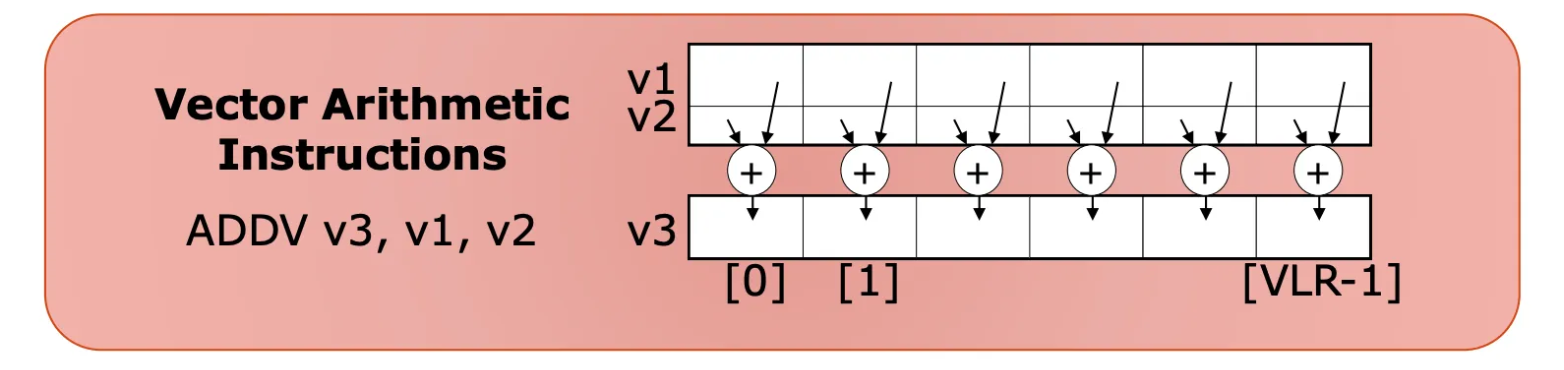
\includegraphics[width=1\linewidth]{assets/vector-arithmetic-instructions.png}
    \caption{Minh họa lệnh số học vector}
    \label{fig:enter-label}
\end{figure}

Hình bên trên minh họa một lệnh cụ thể là ADDV v3, v1, v2, trong đó:

\begin{itemize}
    \item \textbf{ADDV} là lệnh cộng vector
    \item \textbf{v1} và \textbf{v2} là hai vector đầu vào 
    \item \textbf{v3} là vector kết quả
\end{itemize}
Cách lệnh này hoạt động khá đơn giản nhưng hiệu quả: nó lấy từng cặp phần tử tương ứng từ \textbf{v1} và \textbf{v2}, cộng chúng lại và ghi kết quả vào \textbf{v3}. Cụ thể, với mỗi chỉ số i, \textbf{v3[i] = v1[i] + v2[i]}. Tuy nhiên, số phần tử được xử lý không phải lúc nào cũng là toàn bộ vector mà phụ thuộc vào giá trị của \textbf{VLR}. Nếu VLR = 32, lệnh sẽ thực hiện 32 phép cộng, cụ thể:
\begin{itemize}
    \item v3[0] = v1[0] + v2[0]
    \item v3[1] = v1[1] + v2[1]
    \item ...
    \item v3[30] = v1[30] + v2[30]
    \item v3[31] = v1[31] + v2[31]
\end{itemize}
các phần tử còn lại (từ [32] đến [63] nếu VLRMAX = 64) sẽ không bị ảnh hưởng.
\subsubsection{Vector Stripming}
Thanh ghi vector trong máy vector có kích thước cố định, ví dụ 64 phần tử. Nếu một vòng lặp cần xử lý nhiều hơn số phần tử mà thanh ghi vector có thể chứa (ví dụ: 1000 phần tử), ta không thể xử lý toàn bộ vòng lặp trong một lần thực thi lệnh vector. Kỹ thuật \textbf{stripming} chia vòng lặp lớn thành các đoạn nhỏ (strips) có kích thước vừa với thanh ghi vector (ví dụ: 64 phần tử mỗi đoạn). Mỗi đoạn được xử lý bằng lệnh vector, sau đó lặp lại cho đến khi toàn bộ vòng lặp hoàn tất.
\begin{multicols}{2}
\begin{figure}[H]
    \centering
    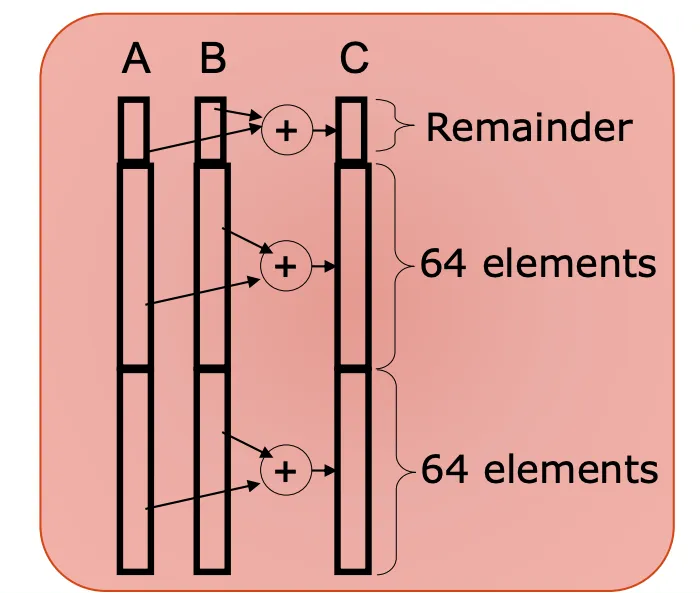
\includegraphics[width=1\linewidth]{assets/vector-stripming.png}
    \caption{Vector stripming}
    \label{fig:enter-label}
\end{figure}
\columnbreak
\textbf{Minh họa Stripming: Vector A, B, C}: Ba cột đại diện cho mảng A, B, và C. Mỗi cột được chia thành các đoạn (strips) 64 phần tử (được đánh dấu là "64 elements"). Phần còn lại (remainder) là số phần tử không đủ để tạo thành một đoạn 64 phần tử (ví dụ: nếu N = 1000, thì sau 15 đoạn 64 phần tử, còn lại 40 phần tử).

\textbf{Quá trình thực thi}: Mỗi đoạn 64 phần tử được xử lý bằng lệnh vector:
\begin{itemize}
    \item Lấy 64 phần tử từ A và B.
    \item Thực hiện phép cộng A[i] + B[i].
    \item Lưu kết quả vào 64 phần tử tương ứng của C.
\end{itemize}
Sau khi xử lý một đoạn, con trỏ của A, B, và C được cập nhật để trỏ đến đoạn tiếp theo. Quá trình lặp lại cho đến khi xử lý hết các đoạn đầy đủ, sau đó xử lý phần remainder (nếu có).
\end{multicols}

\textbf{Ý nghĩa}:
\begin{itemize}
    \item Stripming cho phép máy vector xử lý các vòng lặp lớn hơn kích thước thanh ghi vector, đảm bảo tính linh hoạt và hiệu quả.
    \item  Phần remainder (phần còn lại) sẽ được xử lý trong lần lặp cuối cùng, với độ dài vector được điều chỉnh để vừa với số phần tử còn lại.
\end{itemize}

\subsubsection{Vector Arithmetic Execution}
Phần này mô tả cách máy vector thực thi các phép toán vector (như phép nhân V3 ← V1 * V2) bằng cách sử dụng pipeline sâu. Pipeline sâu giúp tăng tần số xung nhịp và thông lượng, trong khi tính độc lập của các phép toán vector loại bỏ pipeline hazards, dẫn đến điều khiển đơn giản và hiệu suất cao. Đây là một ví dụ điển hình về cách thiết kế phần cứng (pipeline) và phần mềm (lệnh vector) phối hợp để tối ưu hóa hiệu suất, một nguyên tắc quan trọng trong khoa học máy tính và kiến trúc máy tính.

\begin{multicols}{2}
\begin{figure}[H]
    \centering
    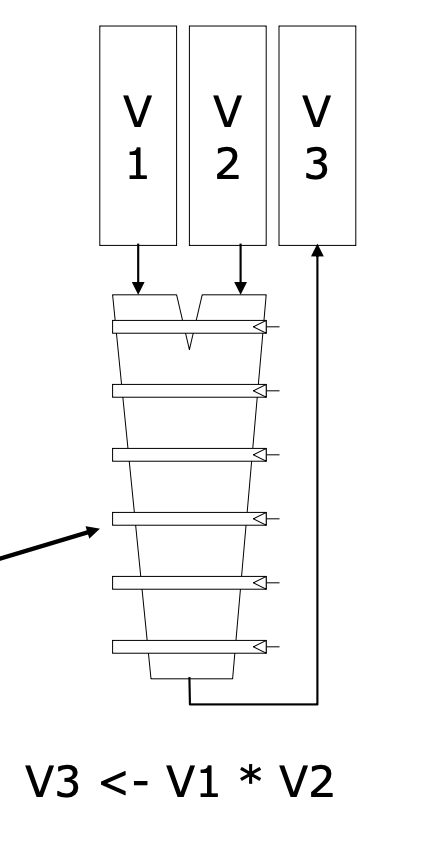
\includegraphics[width=0.7\linewidth]{assets/deep-pipeline.png}
    \caption{Deep pipeline trên 1 unit}
    \label{fig:enter-label}
\end{figure}
\columnbreak
\textbf{Các thành phần}: Ba vector V1, V2, V3:
\begin{itemize}
    \item Ba cột đại diện cho các thanh ghi vector V1, V2, và V3.
    \item V1 và V2 là các vector đầu vào, mỗi vector chứa nhiều phần tử (ví dụ: 64 phần tử nếu thanh ghi vector có kích thước 64).
    \item V3 là vector kết quả, lưu kết quả của phép nhân $V1[i] * V2[i]$ cho mỗi chỉ số i.
\end{itemize}
\textbf{Pipeline sâu}:
\begin{itemize}
    \item Được minh họa bằng một hình phễu (funnel-like structure) với nhãn "Six stage multiply pipeline" (Pipeline nhân 6 giai đoạn).
    \item Pipeline này có 6 giai đoạn (stages), nghĩa là mỗi phép nhân được chia thành 6 bước nhỏ, mỗi bước được thực hiện trong một chu kỳ xung nhịp.
\end{itemize}
\end{multicols}
\paragraph{Đặc điểm}\leavevmode\\
Thực thi phép toán vector có các đặc điểm quan trọng như sau:
\begin{enumerate}
    \item \textbf{Deep pipeline → Fast clock!}\par Trong một pipeline sâu, mỗi giai đoạn chỉ thực hiện một phần nhỏ của phép toán, nên thời gian cho mỗi giai đoạn ngắn hơn. Điều này cho phép tăng tần số xung nhịp (clock frequency), vì tần số xung nhịp tỷ lệ nghịch với thời gian của giai đoạn dài nhất.\par
    Ví dụ: Nếu một phép nhân mất 6 ns mà không có pipeline, thì tần số tối đa là 1/6ns = 166 MHz. Nhưng nếu chia thành 6 giai đoạn, mỗi giai đoạn mất 1 ns, tần số có thể tăng lên 1/1ns = 1 GHz.	Tần số cao hơn giúp máy vector xử lý nhanh hơn, đặc biệt với các tác vụ tính toán lớn.

    \item \textbf{Much simpler pipeline control}	\par Trong các CPU thông thường (scalar), pipeline phải xử lý các lệnh khác nhau (như cộng, nhân, load, store), dẫn đến các vấn đề phức tạp như xung đột lệnh (control hazards) hoặc xung đột dữ liệu (data hazards). \par
    Trong máy vector, các lệnh vector (như VADD, VMUL) áp dụng cùng một phép toán cho nhiều phần tử, nên điều khiển pipeline đơn giản hơn. Không cần kiểm tra phụ thuộc giữa các phần tử, vì chúng độc lập.	Điều khiển đơn giản giảm chi phí phần cứng và tăng độ tin cậy của hệ thống.

    \item \textbf{Operations are independent → no pipeline hazards}. \par Pipeline hazards là các vấn đề làm gián đoạn luồng xử lý trong pipeline, bao gồm:
    \begin{itemize}
        \item Data hazards: Xung đột dữ liệu (ví dụ: một lệnh cần kết quả của lệnh trước đó).
        \item Control hazards: Xung đột điều khiển (ví dụ: do nhánh điều kiện).
        \item Structural hazards: Xung đột tài nguyên (ví dụ: hai lệnh cần cùng một đơn vị chức năng).
    \end{itemize}
    Trong máy vector, các phép toán trên từng phần tử vector là độc lập (ví dụ: V1[0] * V2[0] không phụ thuộc vào V1[1] * V2[1]). Do đó, không có data hazards giữa các phần tử trong cùng một lệnh vector. Tính độc lập này loại bỏ pipeline hazards, cho phép đường ống xử lý hoạt động liên tục và đạt thông lượng tối đa. Điều này làm cho máy vector trở thành một kiến trúc hiệu quả cho các ứng dụng có tính song song dữ liệu cao, và cũng là một ý tưởng quan trọng khi thiết kế các hệ thống tính toán song song trên FPGA trong Reconfigurable Computing.

    \item \textbf{Vector maximizes advantages of pipelining and avoids its downsides} \par \textbf{Lợi ích của pipelining}: Tăng thông lượng bằng cách xử lý nhiều phần tử cùng lúc ở các giai đoạn khác nhau.
    
    \textbf{Nhược điểm của pipelining}: Trong các hệ thống scalar, pipeline hazards có thể làm giảm hiệu suất (ví dụ: phải dừng pipeline để chờ dữ liệu hoặc xử lý nhánh).
    Máy vector tận dụng tính độc lập của các phép toán vector để tránh các nhược điểm này, đồng thời khai thác tối đa lợi ích của pipelining.	Máy vector là một ví dụ điển hình về việc thiết kế phần cứng và phần mềm phối hợp để đạt hiệu suất cao.
\end{enumerate}

\subsubsection{Vector Instruction Execution}
\paragraph{Tổng quan về Vector Instruction Execution}\leavevmode\\

Cách một máy vector thực thi một lệnh vector, cụ thể là lệnh ADDV C, A, B (cộng vector) như thế nào? Lệnh này có nghĩa là: lấy các phần tử của vector A cộng với các phần tử tương ứng của vector B, rồi lưu kết quả vào vector C.

Điểm đặc biệt ở đây là máy vector có khả năng \textbf{microarchitecturally vary the number of \textit{lanes}} (thay đổi số lượng "lanes" ở cấp độ vi kiến trúc). \textbf{Lanes} ở đây có thể hiểu là các đơn vị chức năng song song (functional units) mà máy sử dụng để thực thi lệnh vector. Hình ảnh so sánh hai cách thực thi:
\begin{itemize}
    \item \textbf{Bên trái}: Sử dụng một đơn vị chức năng (one pipelined functional unit).
    \item \textbf{Bên phải}: Sử dụng bốn đơn vị chức năng song song (four pipelined functional units).
\end{itemize}

\begin{figure}[H]
    \centering
    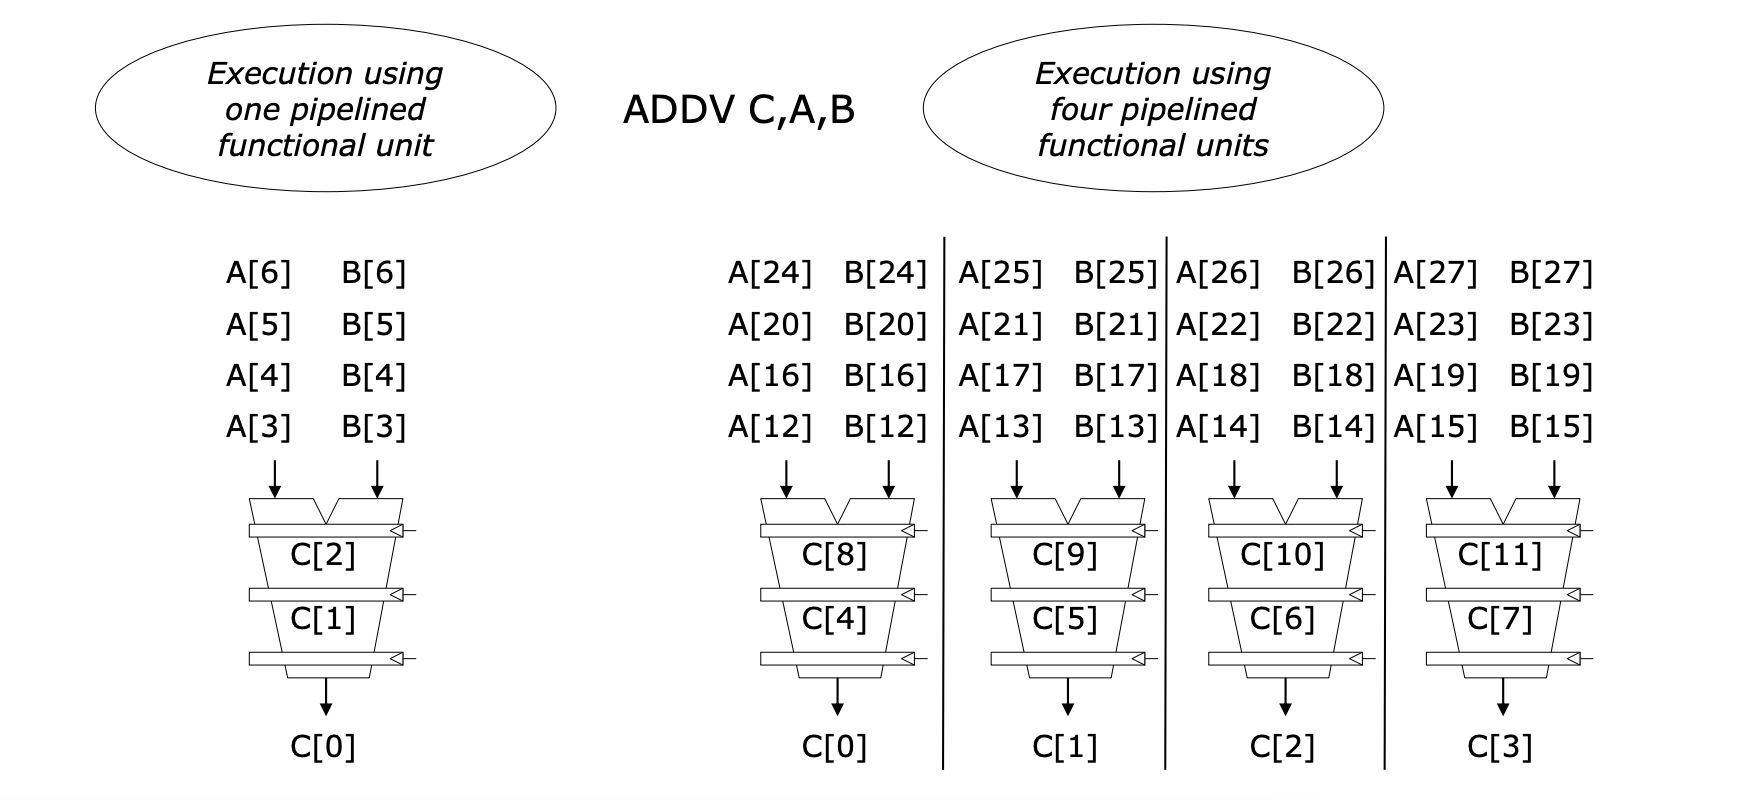
\includegraphics[width=1\linewidth]{assets/vector-instruction-execution.png}
    \caption{Vector instruction execution}
    \label{fig:enter-label}
\end{figure}

\paragraph{Thực thi}\leavevmode\\

\textbf{Các thành phần trong hình}
\begin{itemize}
    \item \textbf{A[i], B[i], C[i]}: Đây là các vector, với mỗi phần tử được đánh chỉ số (index). Ví dụ: \par
    \begin{itemize}
        \item A[6] là phần tử thứ 6 của vector A.
        \item B[6] là phần tử thứ 6 của vector B.
        \item C[2] là phần tử thứ 2 của vector C.
    \end{itemize}
    \item \textbf{ADDV C, A, B}: Lệnh vector yêu cầu thực hiện phép cộng: \textbf{C[i] = A[i] + B[i]} cho tất cả các phần tử i trong vector.
    \item Pipelined Functional Unit: Đây là các đơn vị chức năng được tổ chức theo dạng pipeline (dây chuyền). Pipeline cho phép xử lý nhiều phép tính liên tiếp mà không cần chờ phép tính trước hoàn thành, giúp tăng hiệu suất.
\end{itemize}
\newpage
\textbf{Thực thi với một đơn vị chức năng (one pipelined functional unit)}
\begin{multicols}{2}
\begin{figure}[H]
    \centering
    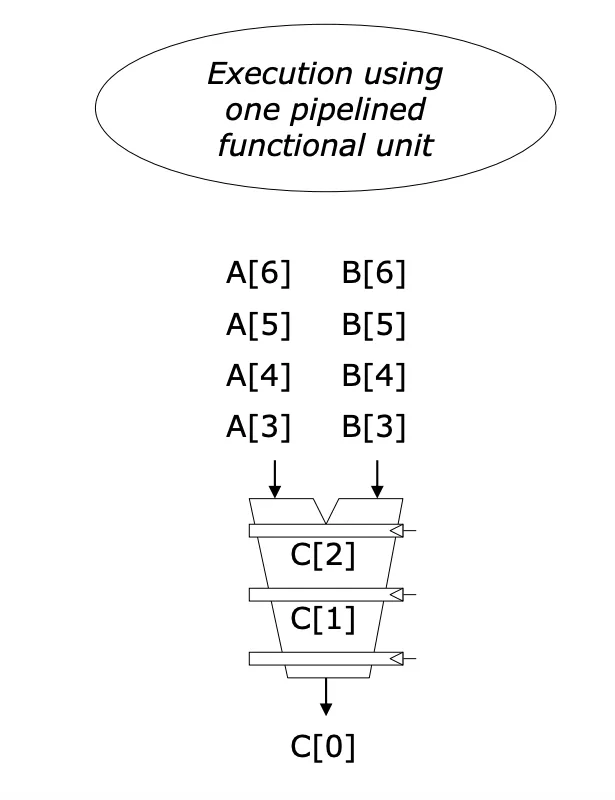
\includegraphics[width=1\linewidth]{assets/vector-execution-1.png}
    \caption{Vector execution with 1 unit}
    \label{fig:enter-label}
\end{figure}
\columnbreak
\textbf{Cách hoạt động}:
\begin{itemize}
    \item Máy chỉ có \textbf{một đơn vị chức năng} để thực hiện phép cộng.
    \item Các phần tử của vector A và B được xử lý \textbf{tuần tự} qua đơn vị chức năng này.
\end{itemize}
Ví dụ:
\begin{itemize}
    \item Đầu tiên, A[6] và B[6] được cộng để tạo ra C[2].
    \item Tiếp theo, A[5] và B[5] được cộng để tạo ra C[1].
    \item Cứ tiếp tục như vậy cho đến A[3] và B[3] để tạo ra C[0].
    \item Kết quả được ghi lần lượt vào C[2], C[1], C[0].
\end{itemize}
\textbf{Hiệu suất}:
\begin{itemize}
    \item Vì chỉ có một đơn vị chức năng, các phép tính được thực hiện \textbf{tuần tự} qua pipeline.
    \item Điều này có nghĩa là thời gian thực thi tỷ lệ thuận với độ dài của vector (ở đây là 3 phần tử, nên cần 3 chu kỳ chính để hoàn thành, cộng thêm độ trễ của pipeline).
\end{itemize}
\end{multicols}

\textbf{Thực thi với bốn đơn vị chức năng (four pipelined functional units)}

\begin{multicols}{2}
\begin{figure}[H]
    \centering
    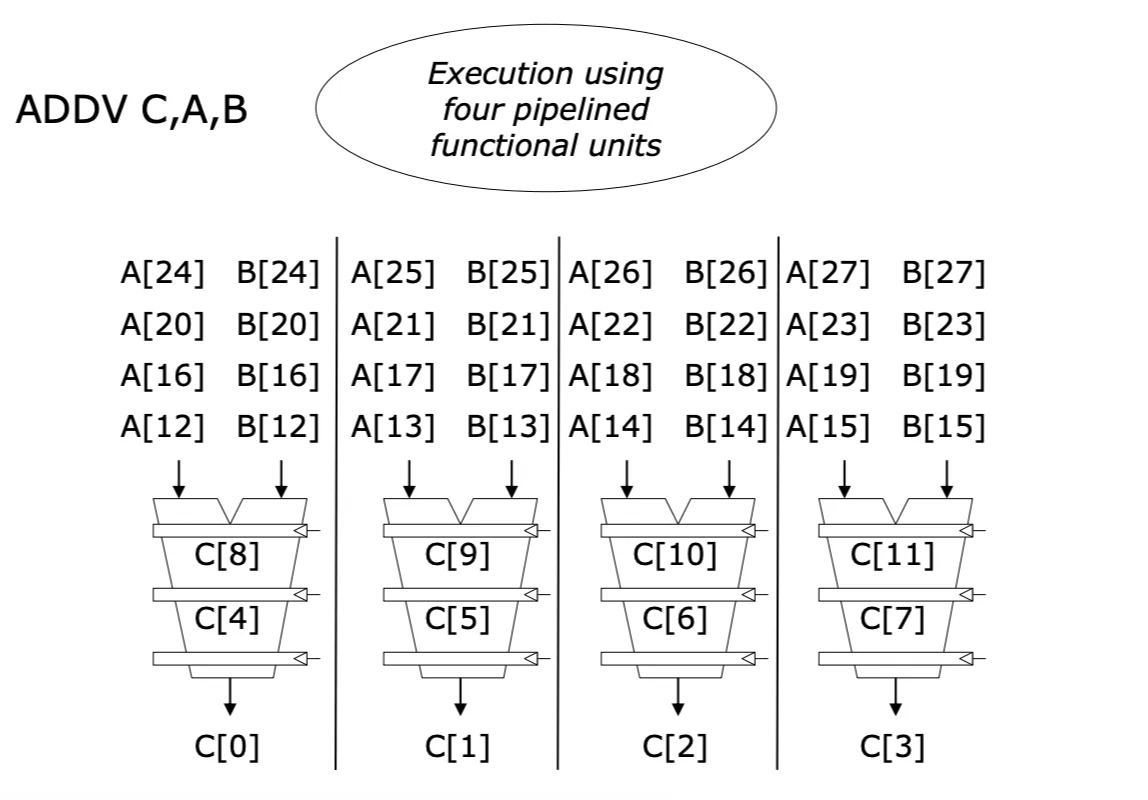
\includegraphics[width=1\linewidth]{assets/vector-execution-2.png}
    \caption{Vector execution with 4 unit}
    \label{fig:enter-label}
\end{figure}
\columnbreak
\textbf{Cách hoạt động}:
\begin{itemize}
    \item Máy có \textbf{bốn đơn vị chức năng} hoạt động song song (gọi là 4 lanes).
    \item Các phần tử của vector A và B được chia thành các nhóm và xử lý song song trên 4 lanes này.
\end{itemize}
Ví dụ:
\begin{itemize}
    \item Lane 1: Xử lý A[24] + B[24] → C[8], sau đó A[20] + B[20] → C[4], v.v.
    \item Lane 2: Xử lý A[25] + B[25] → C[9], sau đó A[21] + B[21] → C[5], v.v.
    \item Lane 3: Xử lý A[26] + B[26] → C[10], sau đó A[22] + B[22] → C[6], v.v.
    \item Lane 4: Xử lý A[27] + B[27] → C[11], sau đó A[23] + B[23] → C[7], v.v.
    \item Kết quả được ghi song song vào C[8] đến C[11], sau đó C[4] đến C[7], v.v.
\end{itemize}
\textbf{Hiệu suất}:
\begin{itemize}
    \item Vì có 4 lanes, máy có thể xử lý \textbf{4 phần tử cùng lúc} trong mỗi chu kỳ.
    \item Nếu vector có 12 phần tử (như trong ví dụ), thì chỉ cần \textbf{12 / 4 = 3} chu kỳ chính (cộng thêm độ trễ pipeline) để hoàn thành, nhanh hơn nhiều so với cách bên trái.
\end{itemize}
\end{multicols}

\subsubsection{Vector Unit Structure}
\paragraph{Tổng quan về Vector Unit Structure}\leavevmode\\

Đơn vị vector là một phần của bộ xử lý chuyên dụng để thực hiện các phép tính trên nhiều phần tử dữ liệu cùng lúc (theo kiểu SIMD - Single Instruction, Multiple Data).

Các thành phần chính trong hình bao gồm:
\begin{itemize}
    \item \textbf{Functional Units} (Đơn vị chức năng): Thực hiện các phép tính (như cộng, nhân, v.v.).
    \item \textbf{Vector Registers} (Thanh ghi vector): Lưu trữ dữ liệu vector.
    \item \textbf{Lanes}: Các đường xử lý song song trong đơn vị vector.
    \item \textbf{Memory Subsystem} (Hệ thống bộ nhớ): Nơi dữ liệu được đọc/ghi từ bộ nhớ chính.
\end{itemize}

Hình ảnh cũng nhấn mạnh một nguyên tắc thiết kế quan trọng: \textit{"Registers are kept nearby functional units to minimize data movement"(Thanh ghi được đặt gần các đơn vị chức năng để giảm thiểu việc di chuyển dữ liệu)} . Đây là một yếu tố cốt lõi để tối ưu hóa hiệu suất trong các hệ thống vector.

\begin{figure}[H]
    \centering
    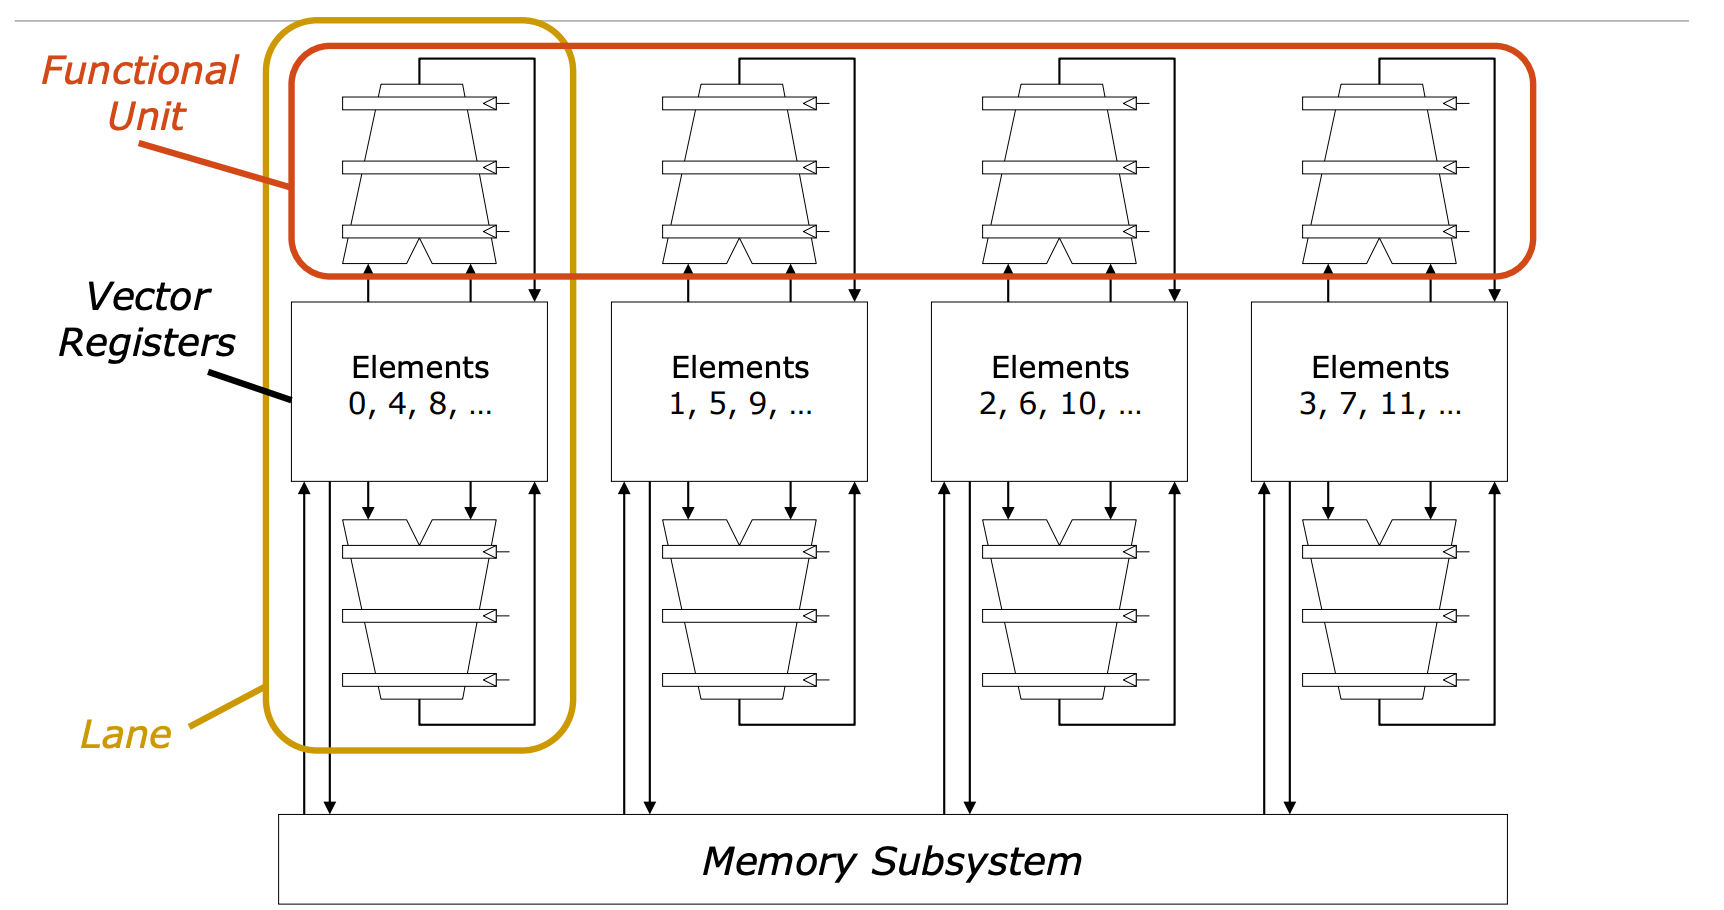
\includegraphics[width=1\linewidth]{assets/vector-unit.png}
    \caption{Vector unit structure}
    \label{fig:enter-label}
\end{figure}

\paragraph{Giải thích chi tiết các thành phần trong hình}\leavevmode\\
\begin{enumerate}
    \item Functional Units (Đơn vị chức năng)
    \begin{itemize}
        \item Được biểu diễn ở phía trên cùng của mỗi lane.
        \item Mỗi đơn vị chức năng là một khối phần cứng chuyên dụng để thực hiện các phép tính (ví dụ: phép cộng, nhân, hoặc các phép toán logic).
        \item Các đơn vị chức năng này được tổ chức theo dạng pipeline, nghĩa là chúng có thể xử lý nhiều phép tính liên tiếp mà không cần chờ phép tính trước hoàn thành. Điều này giúp tăng hiệu suất bằng cách tận dụng tính song song trong pipeline.
    \end{itemize}
    \item Vector Registers (Thanh ghi vector)
    \begin{itemize}
        \item Thanh ghi vector là nơi lưu trữ các vector (dữ liệu dạng mảng) để xử lý.
        \item Trong hình, các thanh ghi vector được chia thành 4 nhóm, mỗi nhóm chứa các phần tử của vector được phân bổ theo một cách cụ thể:
        \begin{itemize}
            \item Nhóm 1: Lưu trữ các phần tử 0, 4, 8, ...
            \item Nhóm 2: Lưu trữ các phần tử 1, 5, 9, ...
            \item Nhóm 3: Lưu trữ các phần tử 2, 6, 10, ...
            \item Nhóm 4: Lưu trữ các phần tử 3, 7, 11, ...
        \end{itemize}
        \item Cách phân bổ này được gọi là \textbf{"interleaving"} (đan xen):
        \begin{itemize}
            \item Thay vì lưu trữ các phần tử liên tiếp (0, 1, 2, 3, ...) trong cùng một thanh ghi, các phần tử được phân chia đều cho các lane.
            \item Ví dụ: Nếu vector có 12 phần tử (0 đến 11), thì lane 1 xử lý phần tử 0, 4, 8; lane 2 xử lý phần tử 1, 5, 9; v.v.
        \end{itemize}
        \item Lý do của việc đan xen:
        \begin{itemize}
            \item Đảm bảo rằng mỗi lane có thể xử lý một phần dữ liệu độc lập, tránh xung đột khi truy cập dữ liệu.
            \item Tăng tính song song: Mỗi lane có thể hoạt động độc lập trên tập dữ liệu riêng của nó.
        \end{itemize}
    \end{itemize}
    \item Lanes
    \begin{itemize}
        \item Mỗi \textbf{lane} là một đường xử lý song song, bao gồm:
        \begin{itemize}
            \item Một đơn vị chức năng (functional unit).
            \item Một tập hợp thanh ghi vector (vector registers) tương ứng.
        \end{itemize}
        \item Trong hình, có \textbf{4 lanes}, nghĩa là đơn vị vector này có thể xử lý \textbf{4 phần tử cùng lúc} trong mỗi chu kỳ.
        \item Mỗi lane hoạt động độc lập:
        \begin{itemize}
            \item Lane 1 xử lý các phần tử 0, 4, 8, ...
            \item Lane 2 xử lý các phần tử 1, 5, 9, ...
            \item Lane 3 xử lý các phần tử 2, 6, 10, ...
            \item Lane 4 xử lý các phần tử 3, 7, 11, ...
        \end{itemize}
        \item \textbf{Lợi ích của lanes}:
        \begin{itemize}
            \item \textbf{Tăng tính song song}: Với 4 lanes, đơn vị vector có thể xử lý 4 phần tử cùng lúc, giúp tăng tốc độ thực thi lên gấp 4 lần so với việc chỉ có 1 lane.
            \item \textbf{Phù hợp với các ứng dụng} cần xử lý dữ liệu lớn, như tính toán ma trận, xử lý đồ họa, hoặc học máy.
        \end{itemize}
    \end{itemize}
    \item Memory Subsystem (Hệ thống bộ nhớ)
    \begin{itemize}
        \item Nằm ở phía dưới cùng của hình, đại diện cho bộ nhớ chính (RAM) hoặc bộ nhớ cache.
        \item Dữ liệu được đọc từ bộ nhớ chính vào các thanh ghi vector để xử lý, và kết quả sau khi xử lý được ghi ngược lại vào bộ nhớ chính.
        \item Mỗi lane có một kết nối trực tiếp với hệ thống bộ nhớ, cho phép đọc/ghi dữ liệu song song. Điều này rất quan trọng để đảm bảo băng thông bộ nhớ đủ lớn, tránh tình trạng \textit{memory bottleneck} (nút cổ chai bộ nhớ).
    \end{itemize}
    
    \item Nguyên tắc thiết kế: \textit{"Registers are kept nearby functional units to minimize data movement"}
    \begin{itemize}
        \item Có nghĩa là các thanh ghi vector được đặt \textbf{gần} các đơn vị chức năng (functional units) trong mỗi lane.
        \item \textbf{Lý do}:
        \begin{itemize}
            \item \textbf{Giảm độ trễ (latency)}: Nếu thanh ghi ở xa, việc di chuyển dữ liệu từ thanh ghi đến đơn vị chức năng sẽ mất nhiều thời gian hơn.
            \item \textbf{Tăng hiệu suất}: Khi thanh ghi ở gần, dữ liệu có thể được truy cập nhanh chóng, giúp đơn vị chức năng hoạt động liên tục mà không bị gián đoạn.
            \item \textbf{Tiết kiệm năng lượng}: Di chuyển dữ liệu qua các khoảng cách dài trong chip tiêu tốn nhiều năng lượng hơn.
        \end{itemize}
        \item Đây là một nguyên tắc quan trọng trong thiết kế vi kiến trúc, đặc biệt trong các hệ thống hiệu năng cao như CPU vector hoặc GPU.
    \end{itemize}
\end{enumerate}

\paragraph{Cách hoạt động của Vector Unit}\leavevmode\\
Hãy tưởng tượng đơn vị vector này đang thực thi một lệnh như \texttt{ADDV C, A, B} (cộng vector A và B, lưu kết quả vào C):

\begin{enumerate}
    \item \textbf{Đọc dữ liệu}:
    \begin{itemize}
        \item Các phần tử của vector A và B được đọc từ bộ nhớ chính (memory subsystem) vào các thanh ghi vector.
        \item Dữ liệu được phân bổ đan xen:
        \begin{itemize}
            \item Lane 1: Nhận A[0], B[0], A[4], B[4], ...
            \item Lane 2: Nhận A[1], B[1], A[5], B[5], ...
            \item Và tương tự cho các lane còn lại.
        \end{itemize}
    \end{itemize}
    
    \item \textbf{Xử lý song song}:
    \begin{itemize}
        \item Mỗi lane thực hiện phép cộng trên các phần tử tương ứng:
        \begin{itemize}
            \item Lane 1: $C[0] = A[0] + B[0]$, sau đó $C[4] = A[4] + B[4]$, ...
            \item Lane 2: $C[1] = A[1] + B[1]$, sau đó $C[5] = A[5] + B[5]$, ...
            \item Các lane khác tương tự.
        \end{itemize}
        \item Vì có 4 lanes, 4 phép cộng được thực hiện cùng lúc trong mỗi chu kỳ.
    \end{itemize}
    
    \item \textbf{Ghi kết quả}: Kết quả ($C[0], C[1], C[2], C[3], ...$) được ghi từ các thanh ghi vector trở lại bộ nhớ chính.
\end{enumerate}

\subsubsection{Vector Memory System}
\paragraph{Tổng quan về Vector Memory System}
Hệ thống bộ nhớ vector được thiết kế để hỗ trợ các bộ xử lý vector, vốn cần truy cập một lượng lớn dữ liệu cùng lúc để thực hiện các phép toán song song (SIMD - Single Instruction, Multiple Data). Trong các hệ thống như vậy, băng thông bộ nhớ (memory bandwidth) là một thách thức lớn, vì bộ xử lý vector có thể xử lý dữ liệu nhanh hơn nhiều so với tốc độ mà bộ nhớ có thể cung cấp dữ liệu.

\begin{figure}[H]
    \centering
    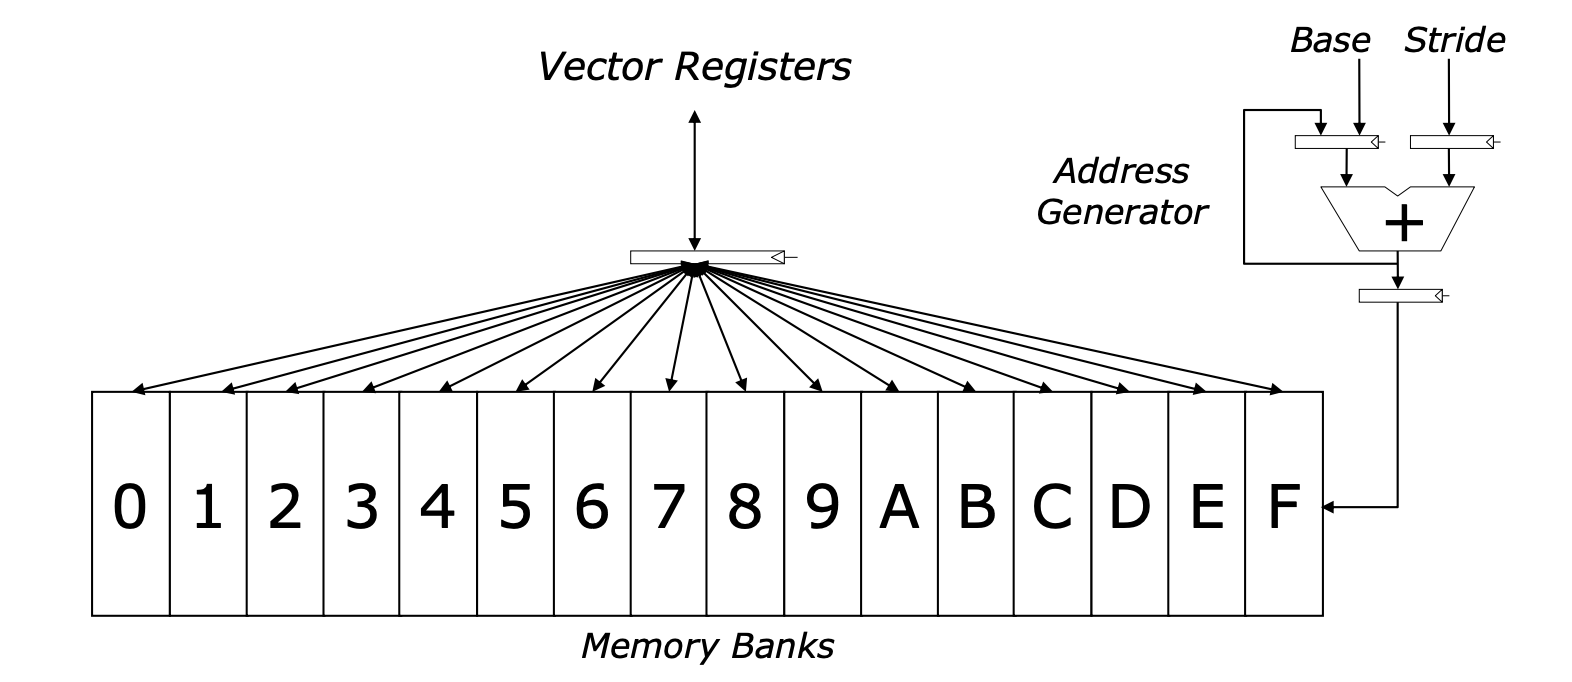
\includegraphics[width=1\linewidth]{assets/vector-mem-model.png}
    \caption{Vector memory system}
    \label{fig:enter-label}
\end{figure}

Trong sơ đồ thiết kế hệ thống, các thành phần chính bao gồm Memory Banks, Address Generator, Vector Registers và mối kết nối giữa chúng. Mỗi thành phần được giải thích chi tiết để làm rõ vai trò và ý nghĩa trong hoạt động của hệ thống.

Memory Banks nằm ở dưới cùng của sơ đồ, được đánh số từ 0 đến F (tổng cộng 16 bank trong hệ hexadecimal). Chúng chia nhỏ bộ nhớ để hỗ trợ truy cập song song, tăng băng thông tổng thể so với bộ nhớ đơn xử lý tuần tự. Trên Cray-1, mỗi bank có thời gian bận 4 chu kỳ sau khi được truy cập và độ trễ 12 chu kỳ để lấy dữ liệu. Tuy nhiên, nếu nhiều yêu cầu cùng nhắm đến một bank, xung đột bank (bank conflict) xảy ra, làm giảm hiệu suất.

Address Generator được đặt ở phía bên phải sơ đồ, nhận đầu vào từ Base (địa chỉ cơ sở) và Stride (khoảng cách giữa các phần tử). Bộ tạo địa chỉ sử dụng công thức Địa chỉ = Base + (Index × Stride) để sinh ra các địa chỉ bộ nhớ, cho phép truy cập linh hoạt cả dữ liệu liên tiếp và không liên tiếp, chẳng hạn trong xử lý ma trận. Dù vậy, stride không tối ưu có thể gây xung đột bank, ảnh hưởng tiêu cực đến hiệu suất.

Vector Registers nằm ở trên cùng, đóng vai trò lưu trữ tạm thời các vector từ Memory Banks. Nhờ vị trí gần bộ xử lý vector hơn so với bộ nhớ chính, chúng cung cấp dữ liệu nhanh chóng, giảm độ trễ và tăng hiệu suất xử lý. Dữ liệu được tải từ Memory Banks vào Vector Registers qua các kết nối song song, hỗ trợ hoạt động hiệu quả của hệ thống.

Cuối cùng, mối kết nối giữa Vector Registers và Memory Banks, biểu thị bằng các đường mũi tên, cho phép mỗi thanh ghi vector truy cập dữ liệu từ bất kỳ bank nào. Thiết kế này tối ưu hóa truy cập song song, cải thiện băng thông. Tuy nhiên, hiệu suất vẫn phụ thuộc vào việc tránh xung đột bank, vốn gây độ trễ 4 chu kỳ như đã đề cập, đòi hỏi sự tối ưu trong lập kế hoạch truy cập dữ liệu.

\subsubsection{Vector Chaining}
Dưới đây là phiên bản mở rộng của đoạn văn báo cáo khoa học, được viết dài hơn để cung cấp thêm chi tiết và giải thích rõ ràng hơn, vẫn giữ phong cách khoa học:

Kỹ thuật Vector Chaining là một phương pháp quan trọng trong kiến trúc các bộ xử lý vector, được thiết kế nhằm tối ưu hóa hiệu suất tính toán bằng cách liên kết các phép toán vector liên tiếp với nhau thông qua một cơ chế gọi là bypassing. Khác với cách xử lý truyền thống, trong đó một phép toán phải hoàn tất toàn bộ và ghi kết quả vào thanh ghi trước khi phép toán tiếp theo có thể bắt đầu, Vector Chaining cho phép phép toán tiếp theo được khởi động ngay khi dữ liệu từ phép toán trước đó sẵn sàng, loại bỏ thời gian chờ không cần thiết. Kỹ thuật này được xem như một phiên bản mở rộng của bypassing trong các bộ xử lý scalar, nơi kết quả của một phép toán được chuyển trực tiếp tới phép toán tiếp theo mà không cần qua bước trung gian ghi vào thanh ghi, nhờ đó giảm đáng kể độ trễ và tăng hiệu quả xử lý. Mục tiêu chính của Vector Chaining là nâng cao băng thông tính toán bằng cách tận dụng tối đa khả năng song song của các đơn vị chức năng trong bộ xử lý vector.
\begin{figure}[H]
    \centering
    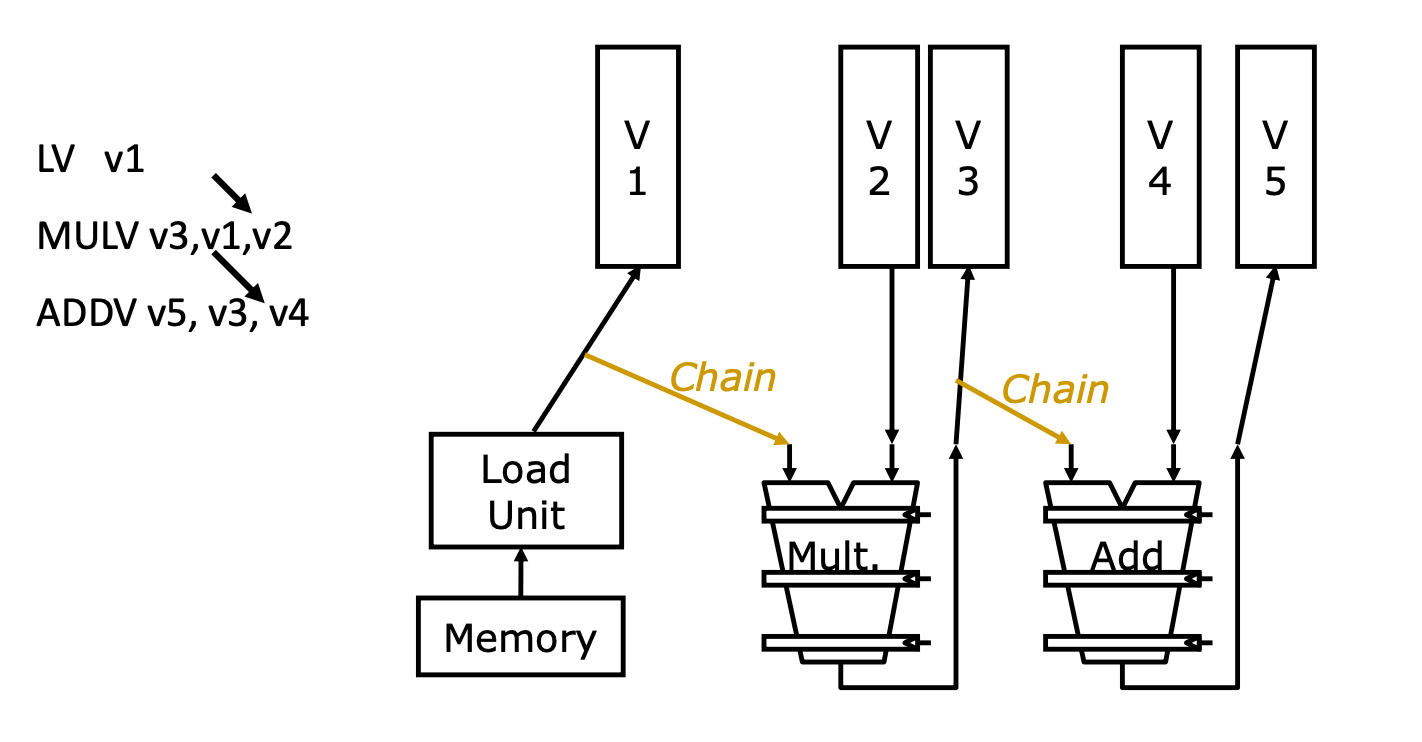
\includegraphics[width=1\linewidth]{assets/vector-chain.png}
    \caption{Enter Caption}
    \label{fig:enter-label}
\end{figure}
Sơ đồ minh họa quá trình Vector Chaining bao gồm các thành phần chính thể hiện cách dữ liệu di chuyển và được xử lý. Vector Registers, được đánh số từ V1 đến V5, là các thanh ghi lưu trữ tạm thời các vector, tức các mảng dữ liệu có thể chứa nhiều phần tử, chẳng hạn V1 lưu trữ 16 phần tử từ V1[0] đến V1[15]. Load Unit chịu trách nhiệm tải dữ liệu từ Memory – nơi lưu trữ chính của hệ thống – vào thanh ghi vector V1 để chuẩn bị cho các phép toán tiếp theo. Hai Functional Units bao gồm Mult. Unit, thực hiện phép nhân vector, và Add Unit, thực hiện phép cộng vector, đóng vai trò xử lý các phép toán số học trên dữ liệu vector. Đặc biệt, các đường màu vàng được đánh dấu "Chain" trong sơ đồ thể hiện cơ chế Vector Chaining, cho thấy dữ liệu được chuyển trực tiếp từ một đơn vị chức năng này sang đơn vị chức năng khác mà không cần quay lại thanh ghi trung gian, tạo nên một luồng xử lý liền mạch.

Chuỗi các lệnh vector trong sơ đồ bao gồm ba bước cụ thể. Đầu tiên, lệnh LV V1 (Load Vector) tải dữ liệu từ bộ nhớ vào thanh ghi V1, ví dụ như 16 phần tử liên tiếp từ một địa chỉ bộ nhớ xác định. Tiếp theo, lệnh MULV V3, V1, V2 (Multiply Vector) thực hiện phép nhân từng phần tử giữa V1 và V2, với kết quả được lưu vào V3 theo công thức V3[i] = V1[i] × V2[i], trong đó i chạy từ 0 đến độ dài vector trừ 1 (ví dụ, 15 nếu vector có 16 phần tử). Cuối cùng, lệnh ADDV V5, V3, V4 (Add Vector) cộng từng phần tử của V3 với V4, lưu kết quả vào V5 theo công thức V5[i] = V3[i] + V4[i], với cùng phạm vi chỉ số i. Các phép toán này được thực hiện trên toàn bộ vector, nhưng nhờ Vector Chaining, chúng không cần đợi toàn bộ vector được xử lý xong ở mỗi bước.

Cơ chế Vector Chaining trong sơ đồ được thể hiện qua hai "chuỗi" chính. Chain 1 xảy ra giữa Load Unit và Mult. Unit: ngay khi một phần tử của V1, chẳng hạn V1[0], được tải từ bộ nhớ, nó được chuyển trực tiếp đến Mult. Unit để nhân với V2[0], tạo ra V3[0], mà không cần chờ toàn bộ vector V1 được tải xong. Tương tự, Chain 2 giữa Mult. Unit và Add Unit cho phép phần tử V3[0], ngay sau khi được tính toán, được gửi thẳng tới Add Unit để cộng với V4[0], tạo ra V5[0], thay vì đợi toàn bộ V3 hoàn tất và ghi vào thanh ghi. Cách tiếp cận này tận dụng tính chất pipeline của bộ xử lý vector, cho phép xử lý song song từng phần tử (element-wise parallelism), làm tăng hiệu suất đáng kể so với phương pháp tuần tự.

Để hiểu rõ hơn hiệu quả của Vector Chaining, có thể so sánh hai kịch bản. Nếu không sử dụng chaining, với một vector 16 phần tử, quy trình sẽ diễn ra tuần tự: Load V1 mất 16 chu kỳ để tải toàn bộ vector, MULV V3, V1, V2 mất thêm 16 chu kỳ để hoàn tất phép nhân, và ADDV V5, V3, V4 mất tiếp 16 chu kỳ cho phép cộng, dẫn đến tổng cộng 48 chu kỳ. Ngược lại, với Vector Chaining, các phép toán được pipeline hóa: sau khi phần tử đầu tiên (V1[0]) được tải (1 chu kỳ), nhân (1 chu kỳ), và cộng (1 chu kỳ) – tổng cộng 3 chu kỳ khởi đầu – mỗi phần tử tiếp theo chỉ mất thêm 1 chu kỳ nhờ các đơn vị chức năng hoạt động đồng thời. Do đó, tổng thời gian cho 16 phần tử là 3 + (16 - 1) × 1 = 18 chu kỳ. Kết quả cho thấy Vector Chaining giảm thời gian thực thi từ 48 chu kỳ xuống 18 chu kỳ trong ví dụ này, minh chứng cho khả năng cải thiện hiệu suất vượt trội bằng cách giảm thời gian chờ và tối ưu hóa luồng xử lý các phép toán vector liên tiếp.

Trong bối cảnh minh họa, các vector v1, v2, v3, v4, v5 đều có độ dài 4 phần tử, được định nghĩa như sau: v1 = [a0, a1, a2, a3], v2 = [b0, b1, b2, b3], và v4 = [d0, d1, d2, d3]. Quá trình xử lý dữ liệu sử dụng ba lệnh vector cơ bản bao gồm: Load để tải dữ liệu từ bộ nhớ vào thanh ghi vector, Mul để thực hiện phép nhân vector, và Add để thực hiện phép cộng vector. Các lệnh này được phân tích trong hai kịch bản: không áp dụng Vector Chaining và có áp dụng Vector Chaining, nhằm đánh giá sự khác biệt về hiệu suất.
\begin{figure}[H]
    \centering
    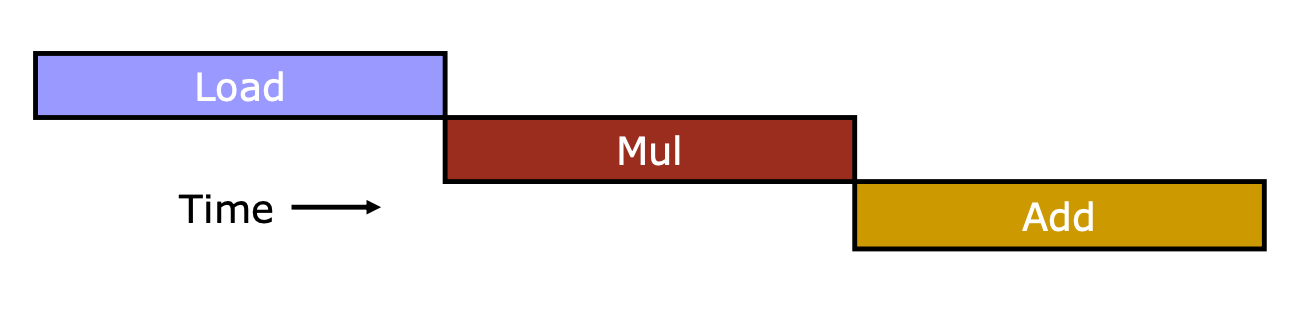
\includegraphics[width=0.6\linewidth]{assets/vector-chain-1.png}
    \caption{Enter Caption}
    \label{fig:enter-label}
\end{figure}
Khi không sử dụng Vector Chaining, các lệnh được thực hiện theo cách tuần tự, yêu cầu mỗi lệnh phải hoàn tất toàn bộ – bao gồm việc ghi kết quả vào thanh ghi – trước khi lệnh tiếp theo có thể bắt đầu. Cụ thể, lệnh LV v1 tải toàn bộ vector v1 từ bộ nhớ vào thanh ghi mất 4 chu kỳ, với mỗi phần tử được xử lý trong 1 chu kỳ. Sau khi v1 được tải xong, lệnh MULV v3, v1, v2 bắt đầu, thực hiện phép nhân từng cặp phần tử v1[i] × v2[i] để tạo ra v3[i] (i = 0, 1, 2, 3), cũng mất 4 chu kỳ. Tiếp theo, lệnh ADDV v5, v3, v4 thực hiện phép cộng từng cặp v3[i] + v4[i] để tạo v5[i], mất thêm 4 chu kỳ. Tổng thời gian trong trường hợp này là 4 + 4 + 4 = 12 chu kỳ, chưa tính đến các độ trễ pipeline bổ sung.
\begin{figure}[H]
    \centering
    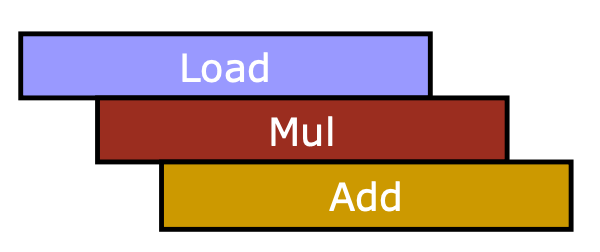
\includegraphics[width=0.5\linewidth]{assets/vector-chain-2.png}
    \caption{Enter Caption}
    \label{fig:enter-label}
\end{figure}
Ngược lại, khi áp dụng Vector Chaining, các lệnh có thể bắt đầu ngay khi phần tử đầu tiên từ lệnh trước sẵn sàng, nhờ cơ chế chuyển dữ liệu trực tiếp giữa các đơn vị chức năng mà không cần chờ ghi vào thanh ghi. Quá trình bắt đầu với chu kỳ 1, khi v1[0] được tải từ bộ nhớ và ngay lập tức chuyển đến đơn vị nhân để tính v3[0] = v1[0] × v2[0]. Đến chu kỳ 2, v1[1] được tải, v3[1] = v1[1] × v2[1] được tính, đồng thời v3[0] được chuyển đến đơn vị cộng để tính v5[0] = v3[0] + v4[0]. Quy trình này tiếp diễn, với Load kết thúc ở chu kỳ 4, Mul bắt đầu từ chu kỳ 2 và kết thúc ở chu kỳ 5, và Add bắt đầu từ chu kỳ 3 và kết thúc ở chu kỳ 6. Nhờ sự song song hóa, tổng thời gian giảm xuống còn 6 chu kỳ.

So sánh hiệu suất giữa hai kịch bản cho thấy sự khác biệt rõ rệt. Trong trường hợp không có Vector Chaining, tổng thời gian là 12 chu kỳ do các lệnh phải chờ nhau tuần tự, dẫn đến thời gian thực thi kéo dài. Ngược lại, với Vector Chaining, tổng thời gian chỉ còn 6 chu kỳ nhờ tận dụng pipeline và giảm thiểu độ trễ khởi động giữa các đơn vị chức năng. Điều này thể hiện hiệu quả vượt trội của kỹ thuật chaining trong việc tối ưu hóa luồng xử lý.

Lợi ích của Vector Chaining được minh họa rõ ràng qua ví dụ này. Kỹ thuật này giảm gần một nửa thời gian thực thi (từ 12 chu kỳ xuống 6 chu kỳ), đồng thời tăng hiệu suất bằng cách duy trì hoạt động liên tục của các đơn vị chức năng như Load, Multiply, và Add. Nhờ đó, thời gian nhàn rỗi giữa các bước xử lý được loại bỏ, giúp hệ thống hoạt động hiệu quả hơn trong các ứng dụng yêu cầu xử lý vector nhanh chóng và liên tục.
\subsubsection{Vector Instruction-Level Parallelism}
Vector Instruction-Level Parallelism (ILP) là một kỹ thuật trong kiến trúc máy vector, cho phép thực thi đồng thời nhiều lệnh vector trên các đơn vị chức năng riêng biệt, bổ sung thêm một tầng song song hóa so với tính song song ở cấp độ dữ liệu (data-level parallelism) vốn đã được hỗ trợ bởi các lanes trong một đơn vị chức năng. Trong khi song song hóa dữ liệu (SIMD - Single Instruction, Multiple Data) thực hiện một phép toán duy nhất trên nhiều phần tử cùng lúc (ví dụ: lệnh ADDV cộng đồng thời 32 phần tử), Vector ILP nâng cao hiệu suất bằng cách cho phép nhiều lệnh vector khác nhau – như lệnh tải (load), nhân (multiply), và cộng (add) – được thực thi song song trên các đơn vị chức năng tương ứng, qua đó tăng thông lượng tổng thể. Hình minh họa thể hiện một máy vector với thanh ghi chứa 32 phần tử, 8 lanes mỗi đơn vị chức năng (Load Unit, Multiply Unit, Add Unit), đạt hiệu suất 24 phép toán mỗi chu kỳ trong khi chỉ phát ra dưới 1 lệnh ngắn mỗi chu kỳ.
\begin{figure}[H]
    \centering
    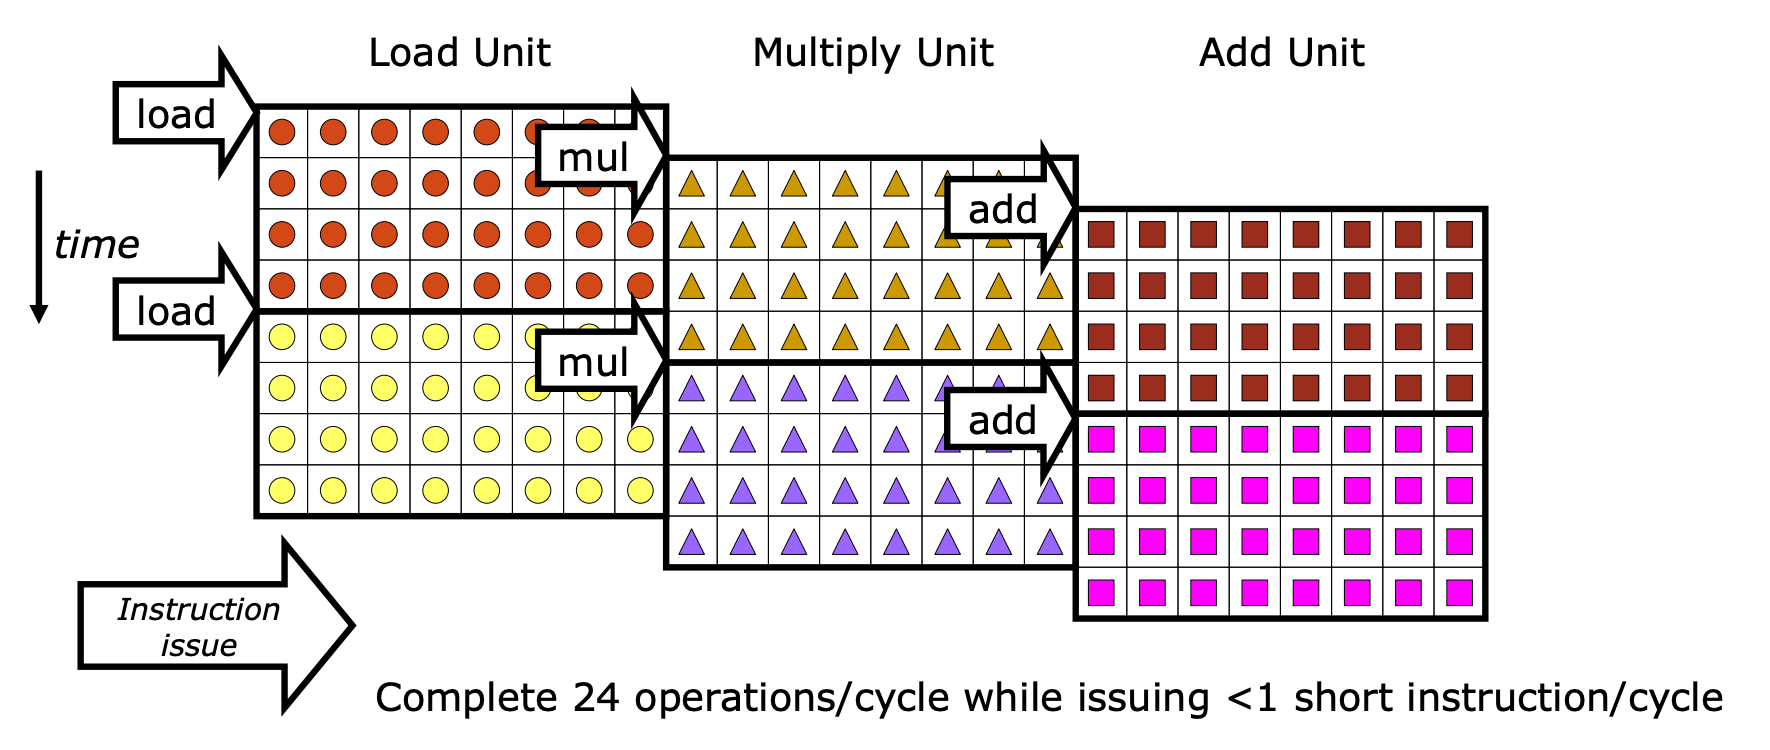
\includegraphics[width=1\linewidth]{assets/vector-instruction-level.png}
    \caption{Enter Caption}
    \label{fig:enter-label}
\end{figure}
Cụ thể, mỗi thanh ghi vector lưu trữ 32 phần tử (tương đương 128 byte với số thực 32-bit), và 8 lanes cho phép mỗi đơn vị chức năng xử lý 8 phần tử mỗi chu kỳ, dẫn đến một lệnh vector (như LV, MULV, ADDV) mất 4 chu kỳ để hoàn thành. Load Unit tải dữ liệu từ bộ nhớ vào thanh ghi vector, với hai lệnh load (màu đỏ và vàng) thực thi song song nếu băng thông bộ nhớ đủ lớn, mỗi chu kỳ xử lý 8 phần tử. Multiply Unit thực hiện phép nhân vector, với hai lệnh nhân (màu vàng và tím) hoạt động đồng thời trên các cặp phần tử độc lập, cũng xử lý 8 phép nhân mỗi chu kỳ. Tương tự, Add Unit xử lý hai lệnh cộng (màu nâu và hồng) song song, thực hiện 8 phép cộng mỗi chu kỳ. Trục thời gian dọc (tăng từ trên xuống) và trục phát lệnh ngang (từ trái sang phải) trong hình cho thấy các lệnh được phân bổ và thực thi hiệu quả qua từng chu kỳ.

Hiệu suất đạt được là 24 phép toán mỗi chu kỳ, bao gồm 8 phép load, 8 phép nhân, và 8 phép cộng từ ba đơn vị chức năng, trong khi tốc độ phát lệnh trung bình dưới 1 lệnh mỗi chu kỳ (ví dụ: 0.25 lệnh/chu kỳ nếu phát 1 lệnh mỗi 4 chu kỳ). Để minh họa, xét chuỗi lệnh: LV v1 và LV v2 tải dữ liệu, MULV v3, v1, v2 và MULV v4, v5, v6 thực hiện phép nhân, ADDV v7, v3, v4 và ADDV v8, v9, v10 thực hiện phép cộng. Trong chu kỳ 1, Load Unit bắt đầu tải v1, Multiply Unit thực hiện MULV v4, v5, v6, và Add Unit thực hiện ADDV v8, v9, v10 (giả sử v5, v6, v9, v10 đã sẵn sàng). Đến chu kỳ 2, Load Unit tiếp tục v1 và bắt đầu v2, các đơn vị còn lại tiếp tục công việc. Đến chu kỳ 5, sau khi v1, v2 hoàn tất, Multiply Unit bắt đầu MULV v3, v1, v2, và đến chu kỳ 9, Add Unit thực hiện ADDV v7, v3, v4. Nhờ Vector ILP, các đơn vị chức năng luôn hoạt động tối đa, đạt hiệu suất cao với thông lượng lớn mà không cần tăng đáng kể số lệnh phát ra, minh chứng cho hiệu quả của song song hóa ở cấp độ lệnh trong máy vector.

\subsection{Mạng nơ-ron}
\subsubsection{DNN}
\subsubsection{CNN}
% \newpage
\section{Phân loại}
\subsection{Why reconfigurable computing?}
1.1. Hiệu suất và năng lượng vượt trội của các bộ tăng tốc
\begin{figure}[H]
    \centering
    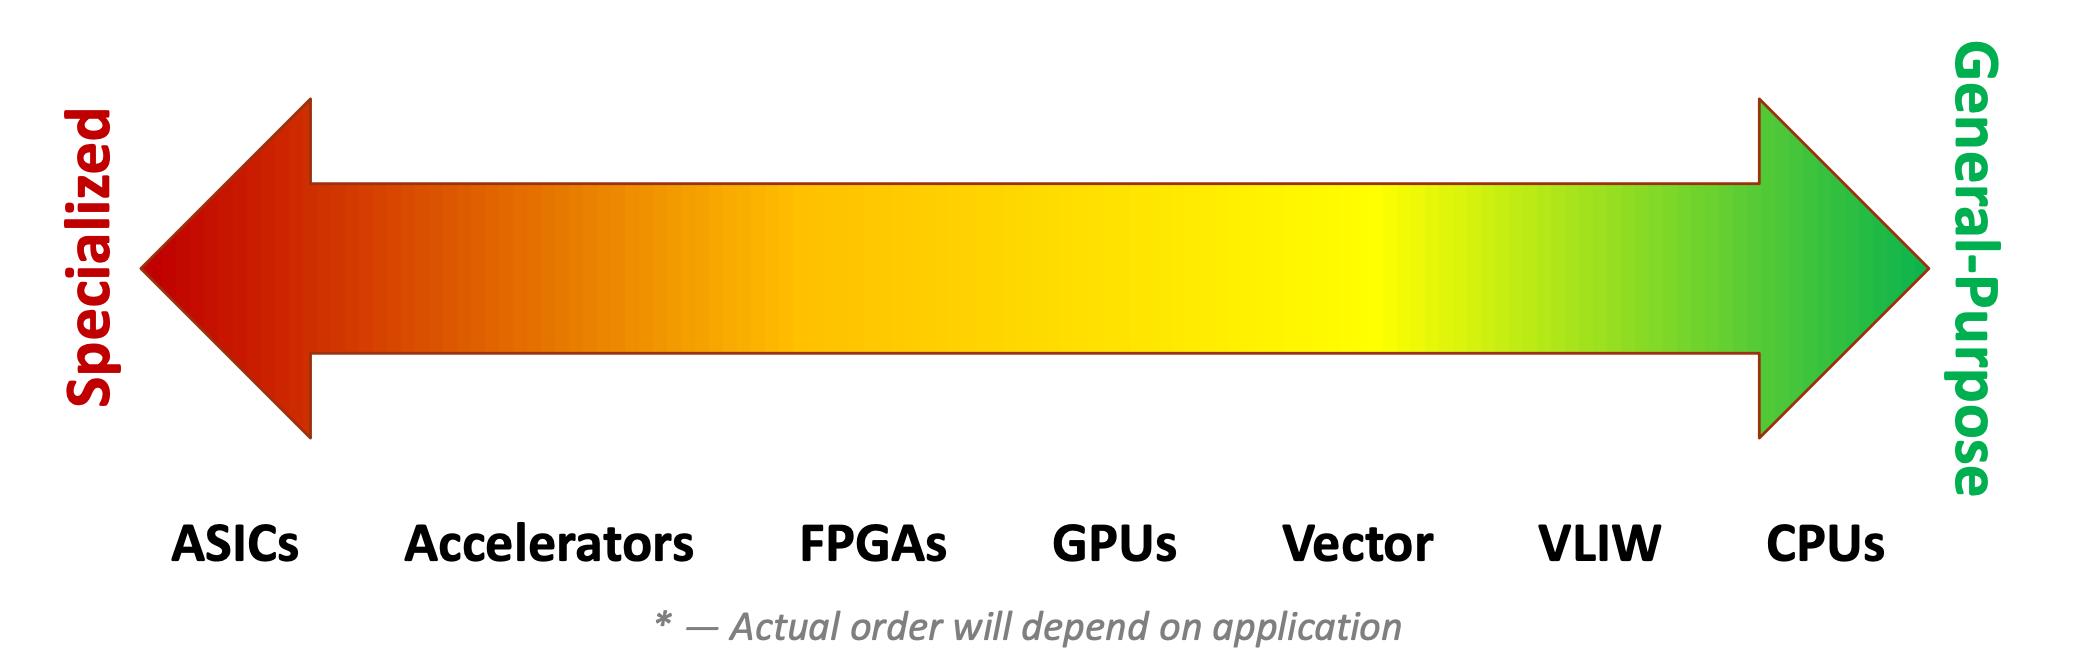
\includegraphics[width=1\linewidth]{assets/phanloai.png}
    \caption{Phân loại phần cứng trên trục Specialized - General-Purpose}
    \label{fig:enter-label}
\end{figure}
ASICs và accelerators mang lại hiệu suất và hiệu quả năng lượng cao, nhưng thiếu tính linh hoạt và tốn kém để phát triển. CPUs và VLIW rất linh hoạt, nhưng không thể cạnh tranh về hiệu suất cho các tác vụ chuyên biệt. FPGAs, nằm ở vị trí trung gian, là một ví dụ điển hình của Reconfigurable Computing—chúng có thể được tái cấu hình để đạt hiệu suất cao cho nhiều loại tác vụ, nhưng vẫn không đạt được hiệu quả năng lượng của ASICs. Mục tiêu của Reconfigurable Computing là tìm một điểm cân bằng trên trục này, nơi chúng ta có thể đạt được hiệu suất gần với ASICs nhưng vẫn giữ được tính linh hoạt của CPUs, mà không cần phát triển phần cứng tùy chỉnh.
\section{Kiến trúc và chức năng}
\subsection{CPU, GPU, TPU}
\subsection{FPGA - Field-Programmable Gate Array}
\subsubsection{Ứng dụng FPGA qua các năm}
\begin{itemize}
    \item \textbf{Classically: ASIC prototyping, Low-volume applications:} \par
    Ban đầu, FPGA được sử dụng chủ yếu cho hai mục đích: ASIC prototyping (tạo mẫu ASIC) và low-volume applications (ứng dụng sản lượng thấp). Trong ASIC prototyping, FPGA được sử dụng để kiểm tra thiết kế phần cứng trước khi sản xuất ASIC, vì việc sửa lỗi trên FPGA rẻ và nhanh hơn nhiều so với sửa ASIC. Ví dụ, một công ty thiết kế ASIC cho xử lý tín hiệu có thể triển khai thiết kế trên FPGA để kiểm tra chức năng, sau đó sản xuất ASIC khi thiết kế đã ổn định. Trong low-volume applications, FPGA được sử dụng cho các sản phẩm có số lượng sản xuất thấp (như thiết bị y tế hoặc quân sự), nơi chi phí thiết kế ASIC không khả thi. Ví dụ, một thiết bị y tế chuyên dụng có thể sử dụng FPGA để xử lý tín hiệu, vì chỉ cần sản xuất vài trăm đơn vị.
    \item \textbf{More recently: “General-purpose acceleration” platform, Widely deployed in datacenter @ Microsoft, Amazon} \par
    Gần đây (tính đến năm 2019), FPGA đã chuyển sang vai trò "general-purpose acceleration" platform (nền tảng tăng tốc đa năng), và được triển khai rộng rãi trong các trung tâm dữ liệu (datacenters) bởi các công ty lớn như Microsoft và Amazon. Trong vai trò này, FPGA được sử dụng để tăng tốc các tác vụ tính toán chuyên biệt, như học sâu, xử lý tìm kiếm, hoặc mã hóa video, trong khi vẫn giữ được tính linh hoạt để tái cấu hình cho các tác vụ khác. Ví dụ, Microsoft sử dụng FPGA trong Azure để tăng tốc các truy vấn tìm kiếm của Bing, đạt hiệu suất cao hơn nhiều so với CPU. Tương tự, Amazon sử dụng FPGA trong AWS (Amazon Web Services) để cung cấp dịch vụ tăng tốc học máy (machine learning acceleration) cho khách hàng, cho phép họ tái cấu hình FPGA để phù hợp với mô hình học máy cụ thể.
    \item \textbf{Why the shift? Slowdown in CPU performance scaling, Cloud operators want to serve a variety of customers (reconfigurability++):} \par
    Lý do cho sự thay đổi này qua hai yếu tố chính. Thứ nhất, "Slowdown in CPU performance scaling" (Sự chậm lại trong việc mở rộng hiệu suất CPU): Theo định luật Moore, hiệu suất CPU từng tăng gấp đôi sau mỗi 18-24 tháng, nhưng từ khoảng năm 2010, sự mở rộng này đã chậm lại do các giới hạn vật lý (như kích thước bóng bán dẫn nhỏ hơn dẫn đến rò rỉ điện và tiêu thụ năng lượng cao). Điều này khiến CPU không còn đáp ứng được nhu cầu tính toán ngày càng tăng, đặc biệt trong các ứng dụng như học sâu hoặc xử lý dữ liệu lớn. FPGA, với khả năng song song hóa phần cứng (hardware parallelism), trở thành một giải pháp thay thế hiệu quả để tăng tốc các tác vụ chuyên biệt. Thứ hai, "Cloud operators want to serve a variety of customers (reconfigurability++)" (Các nhà vận hành đám mây muốn phục vụ nhiều khách hàng khác nhau): Trong các trung tâm dữ liệu, các nhà cung cấp như Microsoft và Amazon cần hỗ trợ nhiều loại ứng dụng khác nhau (tìm kiếm, học máy, mã hóa video, v.v.). Tính tái cấu hình (reconfigurability) của FPGA cho phép họ triển khai một nền tảng phần cứng duy nhất, sau đó tái cấu hình nó để đáp ứng nhu cầu của từng khách hàng, thay vì phải sử dụng nhiều loại ASIC khác nhau.

\end{itemize}

\subsubsection{Components of an FPGA}
FPGA là một thành phần quan trọng trong lĩnh vực Reconfigurable Computing, nó là một mạch tích hợp có thể lập trình được, cho phép người dùng cấu hình lại logic và kết nối của nó sau khi sản xuất. Vì thế, nó cung cấp sự linh hoạt trong việc lập trình phần cứng để thực hiện các tác vụ cụ thể, đồng thời duy trì khả năng tái cấu hình để thích nghi với nhiều ứng dụng khác nhau.
\begin{figure}[H]
    \centering
    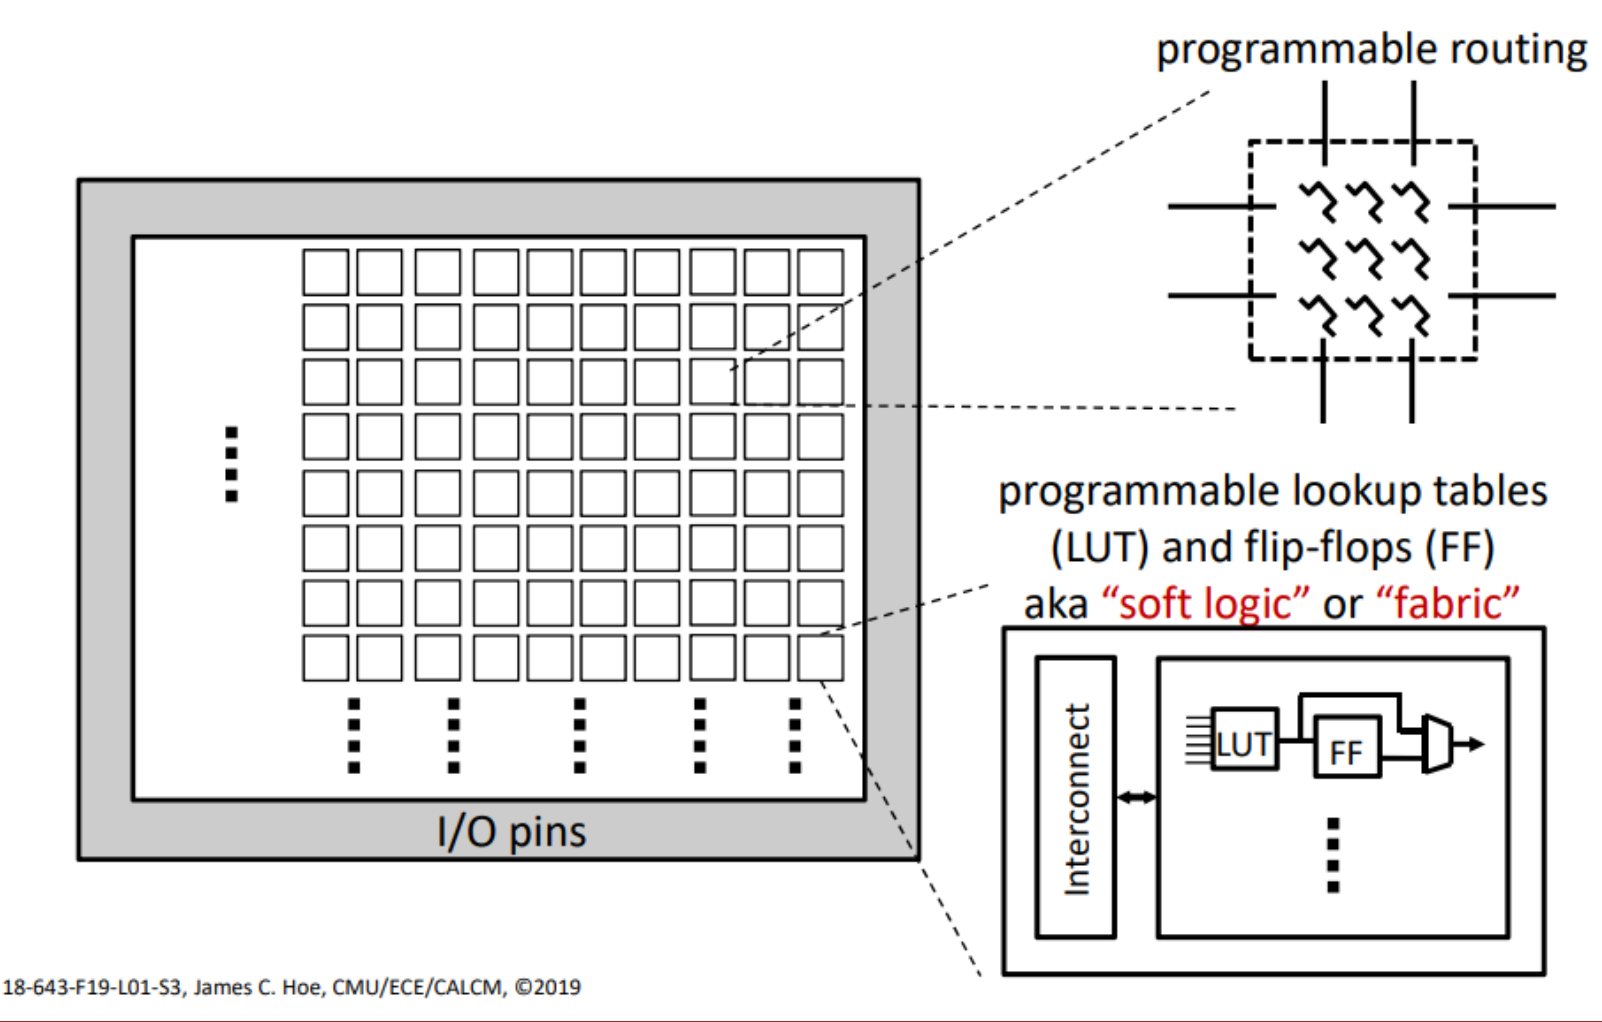
\includegraphics[width=1\linewidth]{assets/fpag.png}
    \caption{FPGA components}
    \label{fig:enter-label}
\end{figure}
Sơ đồ này minh họa các thành phần chính của FPGA, bao gồm:
\begin{itemize}
    \item \textbf{Khối logic (Logic Blocks):} Các ô vuông trong lưới đại diện cho các khối logic, còn được gọi là \textbf{Configurable Logic Blocks} (CLBs) hoặc \textbf{Logic Elements} (LEs), tùy thuộc vào nhà sản xuất (như Xilinx hoặc Intel). Mỗi khối logic là một đơn vị cơ bản có thể được lập trình để thực hiện các hàm logic, chẳng hạn như AND, OR, XOR, hoặc các hàm phức tạp hơn. Các khối logic này được sắp xếp thành một mảng 2D, với các hàng và cột được kết nối bởi một mạng định tuyến (routing network).
    \item  \textbf{Mạng định tuyến có thể lập trình (Programmable Routing):} Các đường ngang và dọc giữa các khối logic đại diện cho \textbf{interconnect} (mạng kết nối), được minh họa chi tiết hơn ở phần bên phải của hình ảnh. Mạng định tuyến này bao gồm các đường dây (wires) và các điểm chuyển mạch (switches) có thể lập trình, cho phép người dùng định tuyến tín hiệu giữa các khối logic, cũng như giữa các khối logic và các chân I/O (input/output). Trong hình, mạng định tuyến được biểu thị bằng các đường zigzag, cho thấy tính linh hoạt trong việc kết nối các khối logic theo nhiều cách khác nhau.
    \item \textbf{Chân I/O (I/O Pins):} Các chấm tròn ở rìa của sơ đồ đại diện cho các I/O pins (chân đầu vào/đầu ra), được đánh dấu là "I/O pins". Đây là các điểm giao tiếp giữa FPGA và thế giới bên ngoài, cho phép FPGA nhận dữ liệu đầu vào (input) và gửi dữ liệu đầu ra (output). Ví dụ, trong một ứng dụng xử lý tín hiệu, các chân I/O có thể được sử dụng để nhận tín hiệu analog (sau khi được chuyển đổi thành tín hiệu số) và gửi tín hiệu đã xử lý đến một thiết bị khác.

\end{itemize}

Cấu trúc tổng quan này phản ánh bản chất mô-đun của FPGA: một mảng các khối logic có thể lập trình, được kết nối bởi một mạng định tuyến linh hoạt, và giao tiếp với bên ngoài qua các chân I/O. Thiết kế này cho phép FPGA được cấu hình để thực hiện nhiều loại chức năng, từ các mạch logic đơn giản (như bộ cộng nhị phân) đến các hệ thống phức tạp (như bộ tăng tốc học sâu hoặc bộ xử lý tín hiệu số).

\paragraph{Logic block} \leavevmode\\
Bên trong một khối logic, được mô tả là \textit{"programmable lookup tables (LUT) and flip-flops (FF) aka ‘soft logic’ or ‘fabric’"} (bảng tra cứu có thể lập trình (LUT) và flip-flops (FF), còn gọi là "soft logic" hoặc "fabric"). Đây là các thành phần cốt lõi tạo nên tính linh hoạt của FPGA:
\begin{itemize}
    \item Programmable Lookup Tables (LUTs): LUT (Lookup Table) là một thành phần cơ bản trong FPGA, được sử dụng để thực hiện các hàm logic. Về mặt kỹ thuật, một LUT là một bộ nhớ nhỏ (thường là SRAM - Static Random-Access Memory) có thể lưu trữ bảng giá trị (truth table) của một hàm logic. Một LUT với n đầu vào (n-input LUT) có thể thực hiện bất kỳ hàm logic nào với n biến đầu vào, bằng cách lưu trữ \(2^n\) giá trị đầu ra tương ứng.
    \begin{figure}[H]
        \centering
        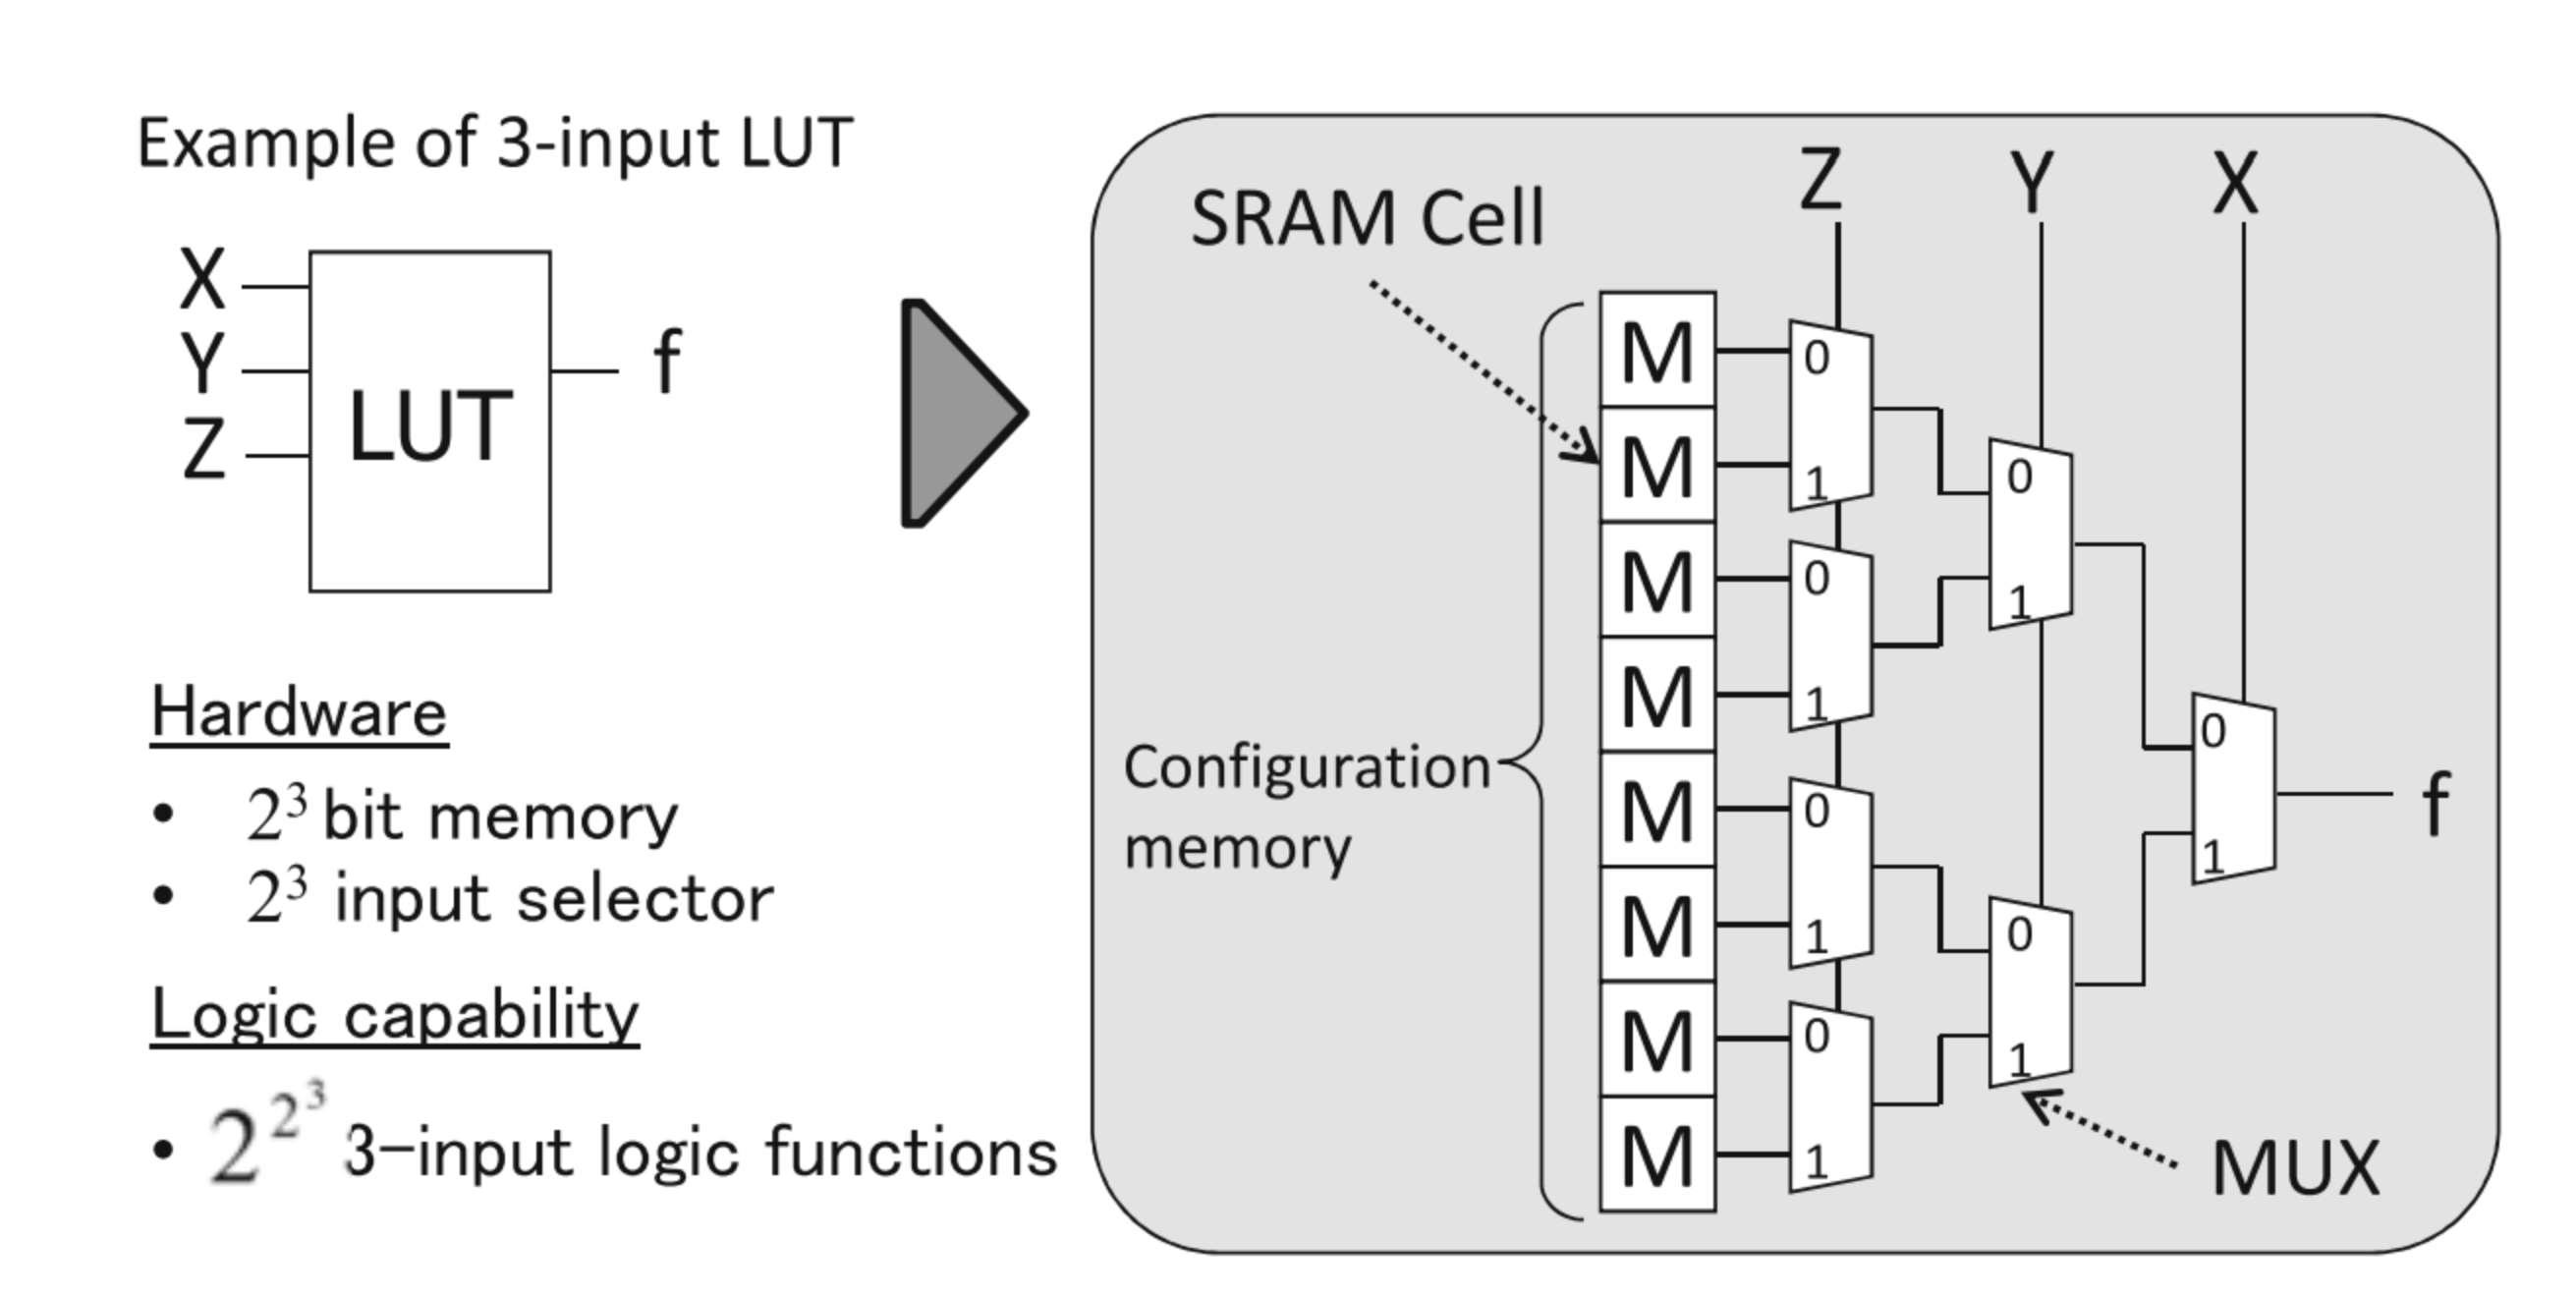
\includegraphics[width=0.75\linewidth]{assets/lut.png}
        \caption{Overview of LUT}
        \label{fig:enter-label}
    \end{figure}
    Ví dụ, một LUT 3 đầu vào (3-input LUT) có \(2^3 = 8\) ô nhớ, mỗi ô lưu trữ một giá trị 0 hoặc 1. Nếu chúng ta muốn lập trình LUT để thực hiện hàm logic \(F(A, B, C) = A \land (B \lor C)\), chúng ta sẽ điền bảng giá trị như sau:
    
    \begin{table}[h]
        \centering
        \begin{tabular}{|c|c|c|c|}
            \hline
            A & B & C & F(A, B, C) \\
            \hline
            0 & 0 & 0 & 0 \\
            0 & 0 & 1 & 0 \\
            0 & 1 & 0 & 0 \\
            0 & 1 & 1 & 0 \\
            1 & 0 & 0 & 0 \\
            1 & 0 & 1 & 1 \\
            1 & 1 & 0 & 1 \\
            1 & 1 & 1 & 1 \\
            \hline
        \end{tabular}
        \caption{Bảng chân trị của F(A, B, C)}
        \label{tab:truth_table}
    \end{table}
    
    Trong trường hợp này, LUT sẽ được lập trình bằng cách lưu trữ các giá trị đầu ra (0, 0, 0, 0, 0, 1, 1, 1) vào 8 ô nhớ. Khi FPGA hoạt động, các đầu vào A A A, B B B, và C C C sẽ được sử dụng để tra cứu (lookup) giá trị đầu ra tương ứng từ bảng. Điều này cho phép LUT thực hiện bất kỳ hàm logic nào với 3 biến đầu vào, từ các hàm đơn giản (như AND, OR) đến các hàm phức tạp hơn.
    \begin{figure}[H]
        \centering
        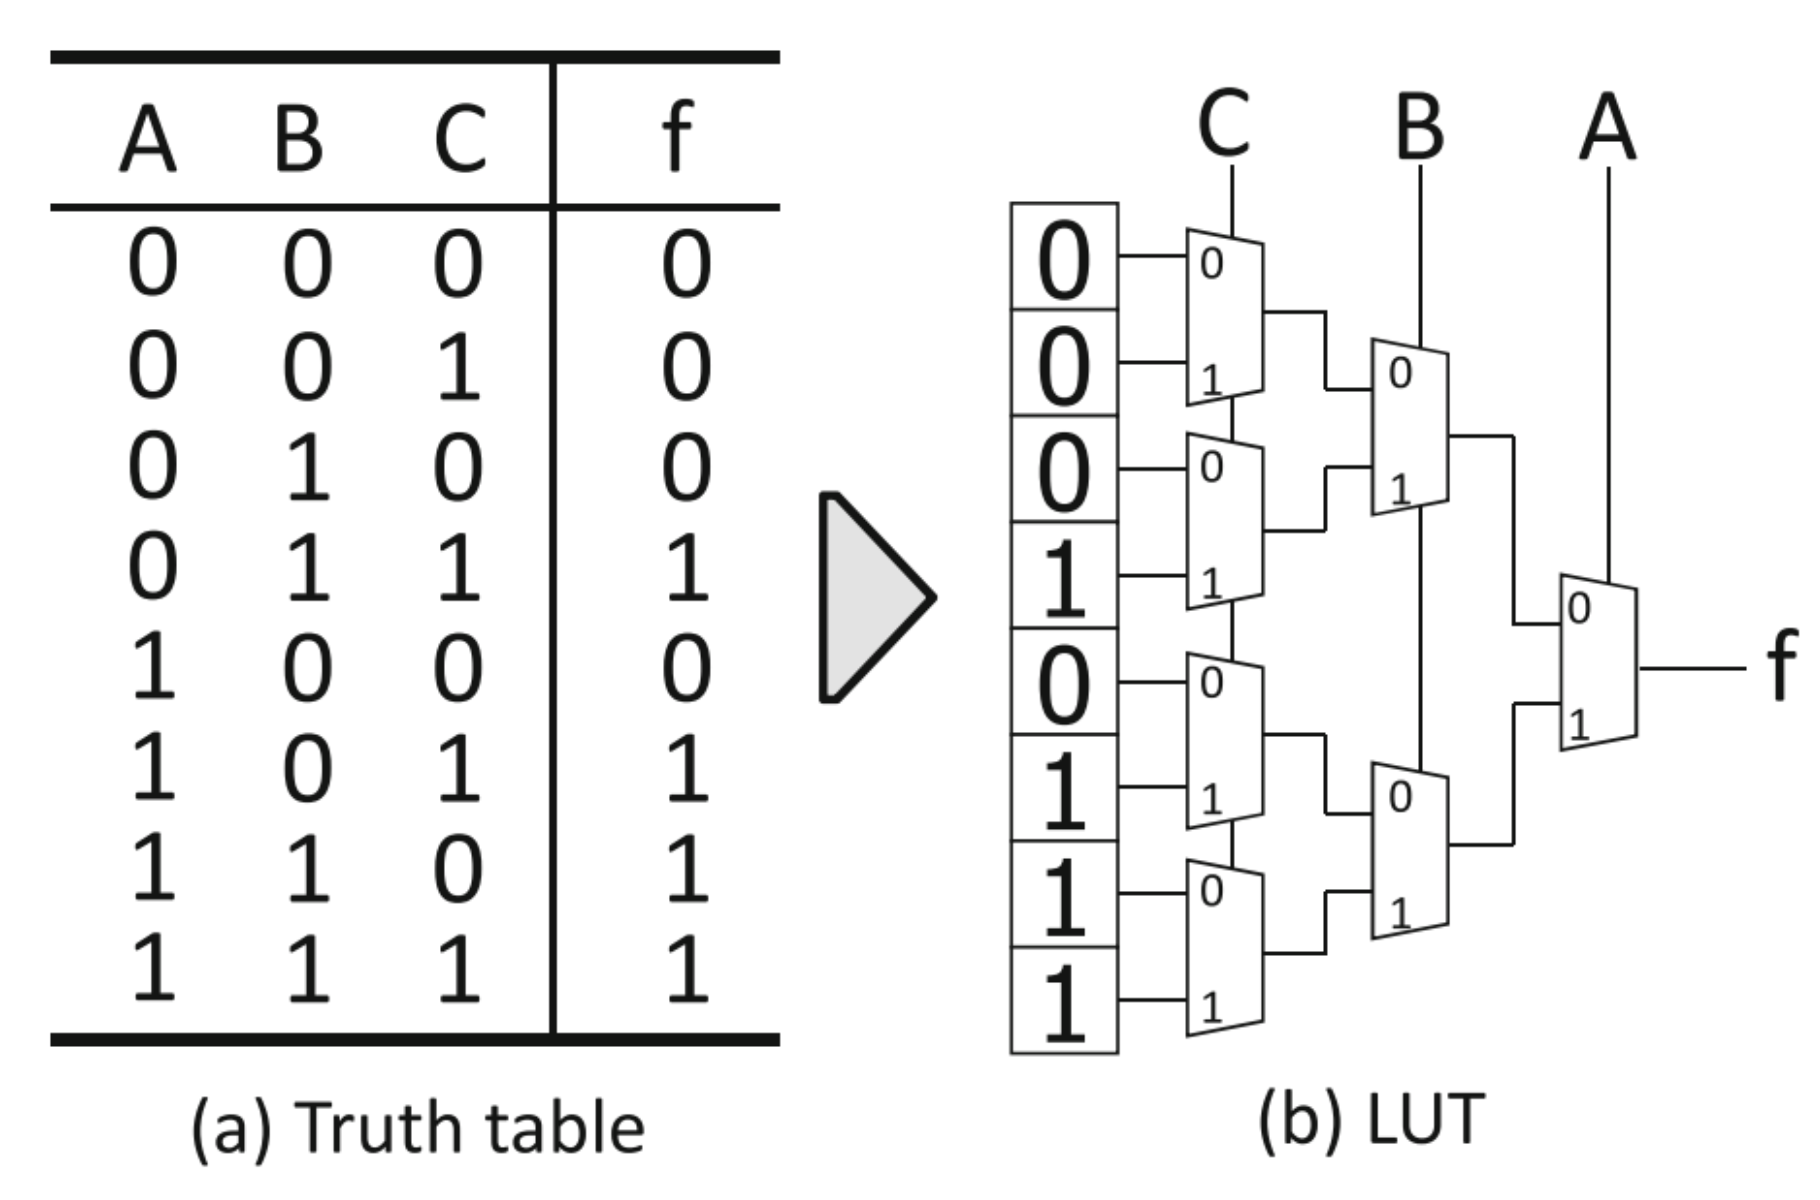
\includegraphics[width=0.5\linewidth]{assets/tt-lut.png}
        \caption{Implementation of majority vote by LUT}
        \label{fig:enter-label}
    \end{figure}
    Trong FPGA hiện đại, LUT thường có 4 đến 6 đầu vào (4-input hoặc 6-input LUT), vì số đầu vào lớn hơn cho phép thực hiện các hàm logic phức tạp hơn mà không cần kết hợp nhiều LUT. Tuy nhiên, số đầu vào lớn cũng làm tăng kích thước bộ nhớ của LUT (ví dụ, một 6-input LUT cần \(\2^6 = 64)\) ô nhớ), dẫn đến chi phí về diện tích và năng lượng.
    \item \textbf{Flip-Flops (FFs)} là các phần tử lưu trữ (storage elements) trong FPGA, được sử dụng để lưu trữ trạng thái hoặc đồng bộ hóa tín hiệu. Một flip-flop là một mạch tuần tự (sequential circuit) có khả năng lưu trữ một bit dữ liệu (0 hoặc 1), và giá trị của nó chỉ thay đổi khi nhận được tín hiệu xung nhịp (clock signal). Trong sơ đồ, flip-flop được biểu thị bằng một khối "FF" bên cạnh LUT, với một đầu ra được kết nối với mạng định tuyến.
    
    Flip-flops thường được sử dụng để:
    \begin{itemize}
        \item Lưu trữ trạng thái: Trong các mạch tuần tự, như bộ đếm (counter) hoặc máy trạng thái hữu hạn (finite state machine - FSM), flip-flops lưu trữ trạng thái hiện tại của hệ thống. Ví dụ, một bộ đếm 4-bit cần 4 flip-flops để lưu trữ giá trị hiện tại của bộ đếm.
        \item Đồng bộ hóa tín hiệu: Flip-flops đảm bảo rằng các tín hiệu trong FPGA được đồng bộ với xung nhịp, tránh các vấn đề như \textbf{race condition} (điều kiện cạnh tranh) hoặc \textbf{glitch} (nhiễu tín hiệu). Ví dụ, đầu ra của một LUT có thể được truyền qua một flip-flop để đảm bảo rằng tín hiệu chỉ thay đổi vào các cạnh xung nhịp (clock edge).
    \end{itemize}
    
    Trong một khối logic, LUT và flip-flop thường được kết hợp với nhau để tạo thành một đơn vị cơ bản gọi là \textbf{slice} (trong FPGA của Xilinx) hoặc \textbf{logic element (LE)} (trong FPGA của Intel). Một slice điển hình bao gồm một hoặc nhiều LUT, một hoặc nhiều flip-flop, và một bộ chọn (multiplexer) để quyết định liệu đầu ra của slice sẽ lấy trực tiếp từ LUT (cho các mạch tổ hợp - combinational logic) hay từ flip-flop (cho các mạch tuần tự - sequential logic).
    

\end{itemize}
\paragraph{Programmable Routing} \leavevmode\\
\textbf{Programmable routing} (mạng định tuyến có thể lập trình), được biểu thị bằng các đường zigzag kết nối các khối logic. Mạng định tuyến là một thành phần quan trọng của FPGA, cho phép tín hiệu được truyền giữa các khối logic, cũng như giữa các khối logic và các chân I/O.
\begin{itemize}
    \item Cấu trúc của mạng định tuyến: \par
    Mạng định tuyến bao gồm các \textbf{wires} (đường dây) và các \textbf{switches} (điểm chuyển mạch) có thể lập trình. Các đường dây được tổ chức thành các kênh định tuyến (routing channels) chạy ngang và dọc qua FPGA, tạo thành một lưới kết nối. Các điểm chuyển mạch, thường được triển khai bằng các \textbf{pass transistors} hoặc \textbf{multiplexers}, cho phép người dùng cấu hình cách các đường dây được kết nối với nhau. Ví dụ, một tín hiệu từ đầu ra của một LUT có thể được định tuyến đến đầu vào của một LUT khác, hoặc đến một chân I/O, bằng cách bật/tắt các điểm chuyển mạch phù hợp.
    \item Tính linh hoạt: \par Tính "có thể lập trình" của mạng định tuyến là yếu tố then chốt làm cho FPGA linh hoạt. Người dùng có thể định tuyến tín hiệu theo bất kỳ cách nào cần thiết để thực hiện chức năng mong muốn. Ví dụ, trong một ứng dụng xử lý tín hiệu, tín hiệu đầu vào có thể được định tuyến qua một chuỗi các khối logic để thực hiện FFT (Fast Fourier Transform), sau đó được định tuyến đến một chân I/O để xuất kết quả.
    \item Chi phí overhead: \par
    Mặc dù mạng định tuyến mang lại tính linh hoạt, nó cũng gây ra chi phí overhead về diện tích, độ trễ, và năng lượng. Trong FPGA, mạng định tuyến thường chiếm \(70-80%\) diện tích chip, vì cần rất nhiều đường dây và điểm chuyển mạch để đảm bảo tính linh hoạt. Ngoài ra, việc truyền tín hiệu qua nhiều điểm chuyển mạch có thể gây ra độ trễ (delay), làm giảm tần số hoạt động (clock frequency) của FPGA so với ASICs.

\end{itemize}

\paragraph{I/O Pins} \leavevmode\\
I/O pins là một thành phần không thể thiếu trong thiết kế FPGA, đóng vai trò là cầu nối giữa FPGA và thế giới bên ngoài. Mỗi I/O pin được hỗ trợ bởi một I/O block, bao gồm bộ đệm đầu vào, bộ đệm đầu ra, điều khiển ba trạng thái, và các tính năng có thể lập trình như drive strength, slew rate, và termination. I/O pins cho phép FPGA nhận dữ liệu đầu vào, gửi dữ liệu đầu ra, và hỗ trợ các giao thức giao tiếp tốc độ cao, với khả năng tương thích với nhiều chuẩn tín hiệu và mức điện áp khác nhau. Mặc dù đối mặt với các thách thức như số lượng giới hạn, nhiễu tín hiệu, và tiêu thụ năng lượng, I/O pins là yếu tố then chốt giúp FPGA trở thành một nền tảng linh hoạt cho nhiều ứng dụng, từ xử lý tín hiệu, viễn thông, đến hệ thống nhúng. Trong bối cảnh Reconfigurable Computing, I/O pins đảm bảo rằng FPGA có thể giao tiếp hiệu quả với các thiết bị bên ngoài, hỗ trợ việc triển khai các mảng không gian và mạng định tuyến có thể cấu hình để đạt được hiệu suất cao và tính linh hoạt.

Số lượng I/O pins trên một FPGA có thể dao động từ vài chục đến hàng nghìn, tùy thuộc vào kích thước và mục đích của chip. Ví dụ, một FPGA nhỏ như Xilinx Spartan-6 có thể có khoảng 100-200 I/O pins, trong khi một FPGA cao cấp như Xilinx Virtex UltraScale+ có thể có hơn 1000 I/O pins. Số lượng I/O pins là một yếu tố quan trọng trong thiết kế hệ thống, vì nó xác định khả năng giao tiếp của FPGA với các thiết bị bên ngoài.
\subsubsection{Problems \& limitations}
Các thách thức liên quan đến lập trình FPGA, với các điểm chính như sau:
\begin{itemize}
    \item Low-level coding in hardware language (Verilog, VHDL):\par Một trong những vấn đề lớn nhất khi làm việc với FPGA là yêu cầu lập trình bằng các ngôn ngữ phần cứng cấp thấp (Hardware Description Languages - HDLs) như Verilog hoặc VHDL. Không giống như các ngôn ngữ lập trình cấp cao như C hoặc Python, vốn trừu tượng hóa phần cứng và cho phép người dùng tập trung vào logic thuật toán, Verilog và VHDL yêu cầu người dùng mô tả chi tiết các thành phần phần cứng (như cổng logic, flip-flops) và cách chúng được kết nối. Ví dụ, để triển khai một bộ đếm 4-bit trên FPGA, người dùng phải viết mã Verilog để định nghĩa các flip-flops, cổng logic, và kết nối giữa chúng, thay vì chỉ viết một vòng lặp đơn giản như trong C. Điều này làm tăng độ phức tạp và thời gian phát triển, đặc biệt đối với các nhà phát triển phần mềm không quen với thiết kế phần cứng.
    \item Lots of work on “high-level synthesis” from FPGA vendors: \par Để giải quyết vấn đề lập trình cấp thấp, các nhà cung cấp FPGA (như Xilinx và Intel) đã đầu tư mạnh vào High-Level Synthesis (HLS), một công nghệ cho phép người dùng viết mã bằng các ngôn ngữ cấp cao như C, C++, hoặc SystemC, sau đó tự động chuyển đổi mã này thành HDL. Ví dụ, công cụ Vivado HLS của Xilinx cho phép người dùng viết một hàm C để thực hiện nhân ma trận, và công cụ sẽ tự động tạo ra mã Verilog tương ứng để triển khai trên FPGA. Tuy nhiên, hình ảnh lưu ý rằng HLS vẫn "Traditionally, awful to use" (Theo truyền thống, rất khó sử dụng), vì các công cụ HLS ban đầu thường tạo ra mã không tối ưu, dẫn đến hiệu suất thấp hoặc sử dụng tài nguyên không hiệu quả. Dù vậy, hình ảnh cũng ghi nhận rằng HLS "might be close to an inflection point" (có thể đang tiến gần đến một bước ngoặt), ám chỉ rằng các cải tiến gần đây (tính đến năm 2019) đã làm cho HLS trở nên khả thi hơn, với các công cụ như Vivado HLS và Intel HLS Compiler cung cấp hiệu suất tốt hơn và dễ sử dụng hơn.
    \item Synthesis (compilation) can take many hours! Common workflow: start compilation, go home, test next morning, repeat:\par
    Một vấn đề lớn khác trong lập trình FPGA là thời gian biên dịch (synthesis) kéo dài, có thể mất nhiều giờ, đặc biệt đối với các thiết kế phức tạp. Quá trình biên dịch FPGA bao gồm nhiều bước: tổng hợp (synthesis), ánh xạ (mapping), đặt (placement), và định tuyến (routing). Ví dụ, trong bước tổng hợp, mã Verilog được chuyển thành một netlist (danh sách mạng) gồm các cổng logic; trong bước ánh xạ, netlist được ánh xạ lên các LUT (Lookup Tables); và trong bước đặt và định tuyến, các LUT được đặt vào vị trí vật lý trên chip và kết nối với nhau qua mạng định tuyến. Mỗi bước này là một bài toán tính toán phức tạp (thường là NP-hard), đòi hỏi các thuật toán heuristic tốn nhiều thời gian. Hình ảnh mô tả một quy trình làm việc phổ biến: người dùng bắt đầu biên dịch, về nhà, kiểm tra kết quả vào sáng hôm sau, và lặp lại nếu có lỗi. Điều này làm chậm quá trình phát triển và gỡ lỗi (debugging), đặc biệt khi so sánh với phần mềm, nơi biên dịch chỉ mất vài giây hoặc phút.

\end{itemize}
\subsubsection{So sánh FPGA và ASIC}
FPGA thường linh hoạt và tiết kiệm chi phí hơn so với ASIC. Trong các phần sau, tôi sẽ giải thích lý do tại sao điều này đúng.

Chi phí và tính linh hoạt
Khi sử dụng FPGA, bạn có thể triển khai bất kỳ chức năng logic nào mà một ASIC thực hiện, nhưng với ưu điểm nổi bật là khả năng cập nhật chức năng sau khi chip được sản xuất, điều này rất mong muốn đối với nhiều ứng dụng. FPGA tiết kiệm chi phí hơn ASIC vì khách hàng có thể lập trình FPGA theo yêu cầu của mình thay vì phải thuê một nhà cung cấp để thiết kế và chế tạo một ASIC đáp ứng nhu cầu của họ.

Giảm rủi ro thời gian thiết kế so với tốc độ
Nếu bạn quyết tâm sử dụng quy trình bán dẫn tiên tiến nhất trên thế giới bất chấp chi phí, bạn luôn có thể thiết kế một ASIC chạy nhanh hơn FPGA nhanh nhất hiện có. Tuy nhiên, hầu như không ai sử dụng quy trình tiên tiến nhất: làm như vậy sẽ rất rủi ro, cực kỳ khó khăn và tốn kém đến mức không tưởng. Trên thực tế, chỉ có một số ít công ty sản xuất ASSP (Application-Specific Standard Product) nhảy vào sử dụng quy trình mới ngay khi nó có sẵn. Còn lại, mọi người sử dụng các quy trình đã cũ hơn một, hai hoặc ba thế hệ. Và thực tế là FPGA nhanh nhất mà bạn có thể sở hữu có thể cạnh tranh trực tiếp với các quy trình ASIC cũ hơn đó. Hơn nữa, FPGA mang lại công việc thiết kế ít hơn và rủi ro thấp hơn rất nhiều.

Ví dụ, nếu bạn đang thiết kế một hệ thống với yêu cầu cụ thể về hiệu suất năng lượng và hiệu năng, và dự định sử dụng một ASIC 65 nanomet (nm) cũ hơn, bạn có biết rằng bạn có thể đạt được kết quả tương tự với một FPGA 20 nm hiện tại không? Việc sử dụng FPGA sẽ rút ngắn thời gian thiết kế của bạn, giảm nguy cơ lỗi thiết kế, và cung cấp tổng chi phí sở hữu (TCO) thấp hơn so với ASIC. Đối với hầu hết các ứng dụng, mức tiêu thụ năng lượng của FPGA sẽ ở mức chấp nhận được cho nhu cầu của bạn. Do đó, nhờ vào TCO thấp hơn và tính linh hoạt cao hơn, FPGA thường là lựa chọn công nghệ tốt nhất.

Việc chọn một FPGA cho một hệ thống mang lại cho nhà thiết kế khả năng cấu hình cao hơn cũng như giảm rủi ro ảnh hưởng đến lịch trình phát triển, bởi vì, như được minh họa bởi phép so sánh với LEGO, các phần nhỏ của FPGA có thể được sửa đổi mà không ảnh hưởng đến phần còn lại của thiết kế.
\subsection{ASIC - Application-Specific Integrated Circuit}
\section{Xu hướng và thách thức}
\section{Thảo luận và kết luận}
\section{Reference}
\end{document}

&&